\documentclass[twoside]{book}

% Packages required by doxygen
\usepackage{fixltx2e}
\usepackage{calc}
\usepackage{doxygen}
\usepackage[export]{adjustbox} % also loads graphicx
\usepackage{graphicx}
\usepackage[utf8]{inputenc}
\usepackage{makeidx}
\usepackage{multicol}
\usepackage{multirow}
\PassOptionsToPackage{warn}{textcomp}
\usepackage{textcomp}
\usepackage[nointegrals]{wasysym}
\usepackage[table]{xcolor}

% Font selection
\usepackage[T1]{fontenc}
\usepackage[scaled=.90]{helvet}
\usepackage{courier}
\usepackage{amssymb}
\usepackage{sectsty}
\renewcommand{\familydefault}{\sfdefault}
\allsectionsfont{%
  \fontseries{bc}\selectfont%
  \color{darkgray}%
}
\renewcommand{\DoxyLabelFont}{%
  \fontseries{bc}\selectfont%
  \color{darkgray}%
}
\newcommand{\+}{\discretionary{\mbox{\scriptsize$\hookleftarrow$}}{}{}}

% Page & text layout
\usepackage{geometry}
\geometry{%
  a4paper,%
  top=2.5cm,%
  bottom=2.5cm,%
  left=2.5cm,%
  right=2.5cm%
}
\tolerance=750
\hfuzz=15pt
\hbadness=750
\setlength{\emergencystretch}{15pt}
\setlength{\parindent}{0cm}
\setlength{\parskip}{0.2cm}
\makeatletter
\renewcommand{\paragraph}{%
  \@startsection{paragraph}{4}{0ex}{-1.0ex}{1.0ex}{%
    \normalfont\normalsize\bfseries\SS@parafont%
  }%
}
\renewcommand{\subparagraph}{%
  \@startsection{subparagraph}{5}{0ex}{-1.0ex}{1.0ex}{%
    \normalfont\normalsize\bfseries\SS@subparafont%
  }%
}
\makeatother

% Headers & footers
\usepackage{fancyhdr}
\pagestyle{fancyplain}
\fancyhead[LE]{\fancyplain{}{\bfseries\thepage}}
\fancyhead[CE]{\fancyplain{}{}}
\fancyhead[RE]{\fancyplain{}{\bfseries\leftmark}}
\fancyhead[LO]{\fancyplain{}{\bfseries\rightmark}}
\fancyhead[CO]{\fancyplain{}{}}
\fancyhead[RO]{\fancyplain{}{\bfseries\thepage}}
\fancyfoot[LE]{\fancyplain{}{}}
\fancyfoot[CE]{\fancyplain{}{}}
\fancyfoot[RE]{\fancyplain{}{\bfseries\scriptsize Generated on Sun Nov 8 2015 16\+:17\+:05 for My Project by Doxygen }}
\fancyfoot[LO]{\fancyplain{}{\bfseries\scriptsize Generated on Sun Nov 8 2015 16\+:17\+:05 for My Project by Doxygen }}
\fancyfoot[CO]{\fancyplain{}{}}
\fancyfoot[RO]{\fancyplain{}{}}
\renewcommand{\footrulewidth}{0.4pt}
\renewcommand{\chaptermark}[1]{%
  \markboth{#1}{}%
}
\renewcommand{\sectionmark}[1]{%
  \markright{\thesection\ #1}%
}

% Indices & bibliography
\usepackage{natbib}
\usepackage[titles]{tocloft}
\setcounter{tocdepth}{3}
\setcounter{secnumdepth}{5}
\makeindex

% Hyperlinks (required, but should be loaded last)
\usepackage{ifpdf}
\ifpdf
  \usepackage[pdftex,pagebackref=true]{hyperref}
\else
  \usepackage[ps2pdf,pagebackref=true]{hyperref}
\fi
\hypersetup{%
  colorlinks=true,%
  linkcolor=blue,%
  citecolor=blue,%
  unicode%
}

% Custom commands
\newcommand{\clearemptydoublepage}{%
  \newpage{\pagestyle{empty}\cleardoublepage}%
}


%===== C O N T E N T S =====

\begin{document}

% Titlepage & ToC
\hypersetup{pageanchor=false,
             bookmarks=true,
             bookmarksnumbered=true,
             pdfencoding=unicode
            }
\pagenumbering{roman}
\begin{titlepage}
\vspace*{7cm}
\begin{center}%
{\Large My Project }\\
\vspace*{1cm}
{\large Generated by Doxygen 1.8.10}\\
\vspace*{0.5cm}
{\small Sun Nov 8 2015 16:17:05}\\
\end{center}
\end{titlepage}
\clearemptydoublepage
\tableofcontents
\clearemptydoublepage
\pagenumbering{arabic}
\hypersetup{pageanchor=true}

%--- Begin generated contents ---
\chapter{Hierarchical Index}
\section{Class Hierarchy}
This inheritance list is sorted roughly, but not completely, alphabetically\+:\begin{DoxyCompactList}
\item \contentsline{section}{Controller\+Parameters2\+D}{\pageref{class_controller_parameters2_d}}{}
\item \contentsline{section}{Controller\+State2\+D}{\pageref{class_controller_state2_d}}{}
\item Mono\+Behaviour\begin{DoxyCompactList}
\item \contentsline{section}{Background\+Parallax}{\pageref{class_background_parallax}}{}
\item \contentsline{section}{Camera\+Controller}{\pageref{class_camera_controller}}{}
\item \contentsline{section}{Character\+Controller2\+D}{\pageref{class_character_controller2_d}}{}
\item \contentsline{section}{Controller\+Physics\+Volume2\+D}{\pageref{class_controller_physics_volume2_d}}{}
\item \contentsline{section}{Follow\+Path}{\pageref{class_follow_path}}{}
\item \contentsline{section}{Jump\+Platform}{\pageref{class_jump_platform}}{}
\item \contentsline{section}{Path\+Definition}{\pageref{class_path_definition}}{}
\item \contentsline{section}{Player}{\pageref{class_player}}{}
\item \contentsline{section}{Sort\+Particle\+System}{\pageref{class_sort_particle_system}}{}
\end{DoxyCompactList}
\end{DoxyCompactList}

\chapter{Class Index}
\section{Class List}
Here are the classes, structs, unions and interfaces with brief descriptions\+:\begin{DoxyCompactList}
\item\contentsline{section}{\hyperlink{class_background_parallax}{Background\+Parallax} \\*klasa \hyperlink{class_background_parallax}{Background\+Parallax} }{\pageref{class_background_parallax}}{}
\item\contentsline{section}{\hyperlink{class_camera_controller}{Camera\+Controller} \\*klasa \hyperlink{class_camera_controller}{Camera\+Controller} }{\pageref{class_camera_controller}}{}
\item\contentsline{section}{\hyperlink{class_character_controller2_d}{Character\+Controller2\+D} \\*klasa \hyperlink{class_character_controller2_d}{Character\+Controller2\+D} }{\pageref{class_character_controller2_d}}{}
\item\contentsline{section}{\hyperlink{class_controller_parameters2_d}{Controller\+Parameters2\+D} \\*klasa \hyperlink{class_controller_parameters2_d}{Controller\+Parameters2\+D} }{\pageref{class_controller_parameters2_d}}{}
\item\contentsline{section}{\hyperlink{class_controller_physics_volume2_d}{Controller\+Physics\+Volume2\+D} \\*klasa \hyperlink{class_controller_physics_volume2_d}{Controller\+Physics\+Volume2\+D} }{\pageref{class_controller_physics_volume2_d}}{}
\item\contentsline{section}{\hyperlink{class_controller_state2_d}{Controller\+State2\+D} \\*klasa \hyperlink{class_controller_state2_d}{Controller\+State2\+D} }{\pageref{class_controller_state2_d}}{}
\item\contentsline{section}{\hyperlink{class_follow_path}{Follow\+Path} \\*klasa \hyperlink{class_follow_path}{Follow\+Path} }{\pageref{class_follow_path}}{}
\item\contentsline{section}{\hyperlink{class_jump_platform}{Jump\+Platform} \\*klasa \hyperlink{class_jump_platform}{Jump\+Platform} }{\pageref{class_jump_platform}}{}
\item\contentsline{section}{\hyperlink{class_path_definition}{Path\+Definition} \\*klasa \hyperlink{class_path_definition}{Path\+Definition} }{\pageref{class_path_definition}}{}
\item\contentsline{section}{\hyperlink{class_player}{Player} \\*klasa \hyperlink{class_player}{Player} }{\pageref{class_player}}{}
\item\contentsline{section}{\hyperlink{class_sort_particle_system}{Sort\+Particle\+System} \\*klasa \hyperlink{class_sort_particle_system}{Sort\+Particle\+System} }{\pageref{class_sort_particle_system}}{}
\end{DoxyCompactList}

\chapter{Class Documentation}
\hypertarget{class_background_parallax}{}\section{Background\+Parallax Class Reference}
\label{class_background_parallax}\index{Background\+Parallax@{Background\+Parallax}}


klasa \hyperlink{class_background_parallax}{Background\+Parallax}  


Inheritance diagram for Background\+Parallax\+:\begin{figure}[H]
\begin{center}
\leavevmode
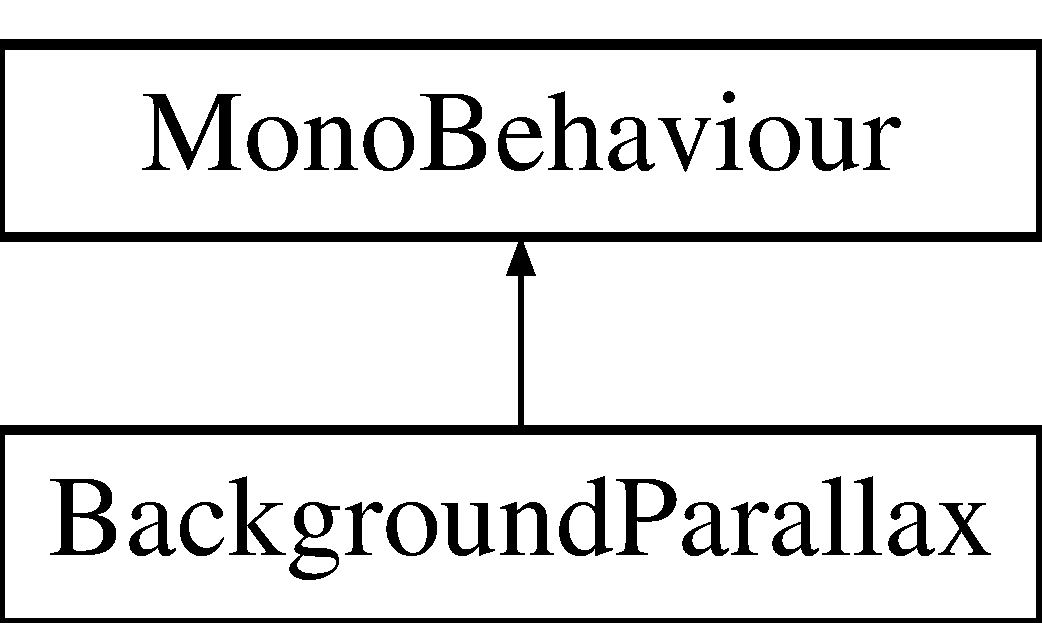
\includegraphics[height=2.000000cm]{class_background_parallax}
\end{center}
\end{figure}
\subsection*{Public Member Functions}
\begin{DoxyCompactItemize}
\item 
void \hyperlink{class_background_parallax_abb5fc2464be1a1bba55238be509a2082}{start} ()
\begin{DoxyCompactList}\small\item\em Zapamiętanie położenia kamery w ostatniej klatce gry, potrzebnego w późniejszym etape do określenia, o ile tło musi się poruszyć w lewo lub prawo. \end{DoxyCompactList}\item 
void \hyperlink{class_background_parallax_a77b333e27f605355ee6b98eb58641ab5}{Update} ()
\begin{DoxyCompactList}\small\item\em Ruch wykonany od ostaniej klatki do obecnej, przeskalowany przez czynnik efektu parallax (intensywności ruchu tła). \end{DoxyCompactList}\end{DoxyCompactItemize}
\subsection*{Public Attributes}
\begin{DoxyCompactItemize}
\item 
Transform\mbox{[}$\,$\mbox{]} \hyperlink{class_background_parallax_a626641e92b9bedfbd0f5aaf2938875b3}{Backgrounds}
\begin{DoxyCompactList}\small\item\em Tablica rzędów elementów tła. \end{DoxyCompactList}\item 
float \hyperlink{class_background_parallax_a078a366dfc612de0f0848b9be330f055}{Parallax\+Scale}
\begin{DoxyCompactList}\small\item\em Wartość efektu poruszania się tła. \end{DoxyCompactList}\item 
float \hyperlink{class_background_parallax_aad6f6a27f24a5d911991227f8abe1a71}{Parallax\+Reduction\+Factor}
\begin{DoxyCompactList}\small\item\em Wartość redukująca stopień poruszania się, dla warstw (rzędów elementów) dalej położonych. \end{DoxyCompactList}\item 
float \hyperlink{class_background_parallax_ad9e09d728695d0c26f103ee614b67000}{Smoothing}
\begin{DoxyCompactList}\small\item\em Zapewnienie płynności ruchu. \end{DoxyCompactList}\end{DoxyCompactItemize}


\subsection{Detailed Description}
klasa \hyperlink{class_background_parallax}{Background\+Parallax} 



\subsection{Member Function Documentation}
\hypertarget{class_background_parallax_abb5fc2464be1a1bba55238be509a2082}{}\index{Background\+Parallax@{Background\+Parallax}!start@{start}}
\index{start@{start}!Background\+Parallax@{Background\+Parallax}}
\subsubsection[{start()}]{\setlength{\rightskip}{0pt plus 5cm}void Background\+Parallax.\+start (
\begin{DoxyParamCaption}
{}
\end{DoxyParamCaption}
)}\label{class_background_parallax_abb5fc2464be1a1bba55238be509a2082}


Zapamiętanie położenia kamery w ostatniej klatce gry, potrzebnego w późniejszym etape do określenia, o ile tło musi się poruszyć w lewo lub prawo. 

\hypertarget{class_background_parallax_a77b333e27f605355ee6b98eb58641ab5}{}\index{Background\+Parallax@{Background\+Parallax}!Update@{Update}}
\index{Update@{Update}!Background\+Parallax@{Background\+Parallax}}
\subsubsection[{Update()}]{\setlength{\rightskip}{0pt plus 5cm}void Background\+Parallax.\+Update (
\begin{DoxyParamCaption}
{}
\end{DoxyParamCaption}
)}\label{class_background_parallax_a77b333e27f605355ee6b98eb58641ab5}


Ruch wykonany od ostaniej klatki do obecnej, przeskalowany przez czynnik efektu parallax (intensywności ruchu tła). 

Dla każdej warstwy (rzędu elementów) tła.

Zapamiętanie pozycji warstwy tła uaktualnionej o efekt parallax,

oraz postepującą redukcję tego efektu dla coraz dalszych warstw.

Ustawienie aktualnej pozycji warstw tła.

Obecna pozycja tła.

Nowa pozycja tła.

Określony efekt płynności animacji efektu w grze.

Uaktualnienie ruchu kamery. 

\subsection{Member Data Documentation}
\hypertarget{class_background_parallax_a626641e92b9bedfbd0f5aaf2938875b3}{}\index{Background\+Parallax@{Background\+Parallax}!Backgrounds@{Backgrounds}}
\index{Backgrounds@{Backgrounds}!Background\+Parallax@{Background\+Parallax}}
\subsubsection[{Backgrounds}]{\setlength{\rightskip}{0pt plus 5cm}Transform \mbox{[}$\,$\mbox{]} Background\+Parallax.\+Backgrounds}\label{class_background_parallax_a626641e92b9bedfbd0f5aaf2938875b3}


Tablica rzędów elementów tła. 

\hypertarget{class_background_parallax_aad6f6a27f24a5d911991227f8abe1a71}{}\index{Background\+Parallax@{Background\+Parallax}!Parallax\+Reduction\+Factor@{Parallax\+Reduction\+Factor}}
\index{Parallax\+Reduction\+Factor@{Parallax\+Reduction\+Factor}!Background\+Parallax@{Background\+Parallax}}
\subsubsection[{Parallax\+Reduction\+Factor}]{\setlength{\rightskip}{0pt plus 5cm}float Background\+Parallax.\+Parallax\+Reduction\+Factor}\label{class_background_parallax_aad6f6a27f24a5d911991227f8abe1a71}


Wartość redukująca stopień poruszania się, dla warstw (rzędów elementów) dalej położonych. 

\hypertarget{class_background_parallax_a078a366dfc612de0f0848b9be330f055}{}\index{Background\+Parallax@{Background\+Parallax}!Parallax\+Scale@{Parallax\+Scale}}
\index{Parallax\+Scale@{Parallax\+Scale}!Background\+Parallax@{Background\+Parallax}}
\subsubsection[{Parallax\+Scale}]{\setlength{\rightskip}{0pt plus 5cm}float Background\+Parallax.\+Parallax\+Scale}\label{class_background_parallax_a078a366dfc612de0f0848b9be330f055}


Wartość efektu poruszania się tła. 

\hypertarget{class_background_parallax_ad9e09d728695d0c26f103ee614b67000}{}\index{Background\+Parallax@{Background\+Parallax}!Smoothing@{Smoothing}}
\index{Smoothing@{Smoothing}!Background\+Parallax@{Background\+Parallax}}
\subsubsection[{Smoothing}]{\setlength{\rightskip}{0pt plus 5cm}float Background\+Parallax.\+Smoothing}\label{class_background_parallax_ad9e09d728695d0c26f103ee614b67000}


Zapewnienie płynności ruchu. 



The documentation for this class was generated from the following file\+:\begin{DoxyCompactItemize}
\item 
C\+:/\+Users/\+Paul/\+Projects/\+Unity\+Game/\+Projekt/\+Assets/\+Code/Background\+Parallax.\+cs\end{DoxyCompactItemize}

\hypertarget{class_camera_controller}{}\section{Camera\+Controller Class Reference}
\label{class_camera_controller}\index{Camera\+Controller@{Camera\+Controller}}


klasa \hyperlink{class_camera_controller}{Camera\+Controller}  


Inheritance diagram for Camera\+Controller\+:\begin{figure}[H]
\begin{center}
\leavevmode
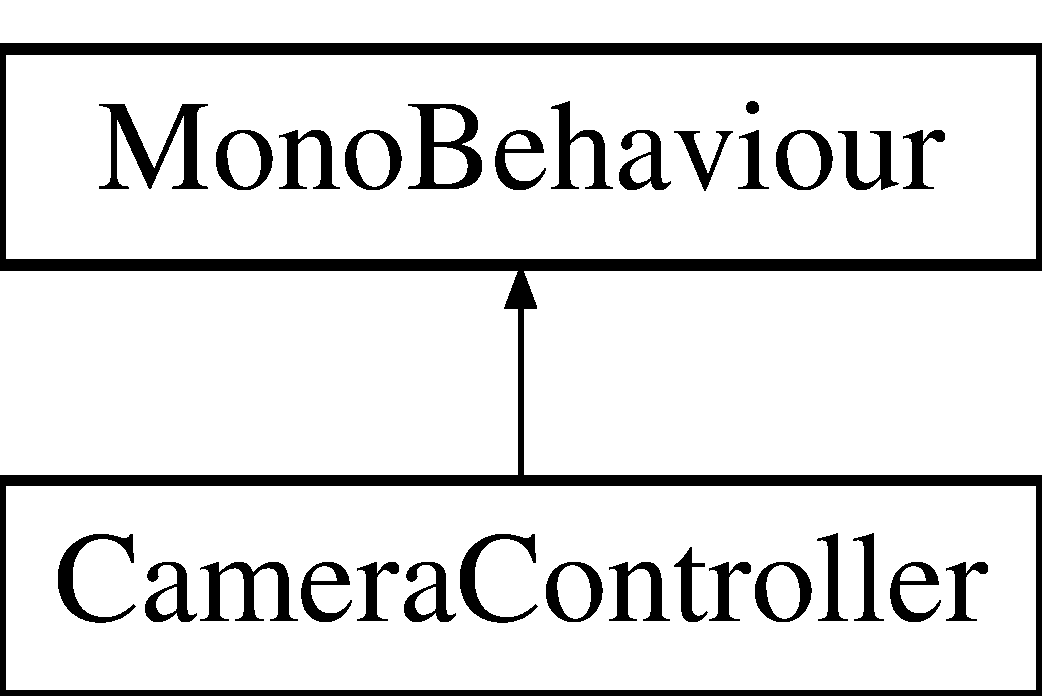
\includegraphics[height=2.000000cm]{class_camera_controller}
\end{center}
\end{figure}
\subsection*{Public Member Functions}
\begin{DoxyCompactItemize}
\item 
void \hyperlink{class_camera_controller_ad4a238c6f7db3ee003302a245d860860}{Start} ()
\begin{DoxyCompactList}\small\item\em Ustawienie ograniczeń rozmiaru obszaru, w którym może się poruszać kamera, oraz ustawienie podążania kamery za graczem. \end{DoxyCompactList}\item 
void \hyperlink{class_camera_controller_a7c4f486f4bcbd1d54a346fdce9707bd5}{Update} ()
\begin{DoxyCompactList}\small\item\em Metoda Update \end{DoxyCompactList}\end{DoxyCompactItemize}
\subsection*{Public Attributes}
\begin{DoxyCompactItemize}
\item 
Transform \hyperlink{class_camera_controller_a0028f1f6c8d940c36cfb6f6ea77b8658}{Player}
\begin{DoxyCompactList}\small\item\em Obiekt gracza. \end{DoxyCompactList}\item 
Vector2 \hyperlink{class_camera_controller_a8c93ba738eeff2eb5af4bc2bc4ec3f10}{Margin}
\begin{DoxyCompactList}\small\item\em Wartość progu ruchu gracza, od którego ma nastapić zmiana położenia kamery. \end{DoxyCompactList}\item 
Vector2 \hyperlink{class_camera_controller_aaa266990dfb97f6e19d4dd6489f683ef}{Smoothing}
\begin{DoxyCompactList}\small\item\em Zapewnienie płynności ruchu kamery. \end{DoxyCompactList}\item 
Box\+Collider2\+D \hyperlink{class_camera_controller_aad472aa9d9410f6b05884b0d4d336d45}{Bounds}
\begin{DoxyCompactList}\small\item\em Ograniczenia ruchu kamery w świecie gry. \end{DoxyCompactList}\end{DoxyCompactItemize}
\subsection*{Properties}
\begin{DoxyCompactItemize}
\item 
bool \hyperlink{class_camera_controller_a1eb503b3ec9f5c4b2f267e859ba37467}{Is\+Following}\hspace{0.3cm}{\ttfamily  \mbox{[}get, set\mbox{]}}
\begin{DoxyCompactList}\small\item\em Zmienna, mówiąca, czy kamera podąża za graczem. \end{DoxyCompactList}\end{DoxyCompactItemize}


\subsection{Detailed Description}
klasa \hyperlink{class_camera_controller}{Camera\+Controller} 



\subsection{Member Function Documentation}
\hypertarget{class_camera_controller_ad4a238c6f7db3ee003302a245d860860}{}\index{Camera\+Controller@{Camera\+Controller}!Start@{Start}}
\index{Start@{Start}!Camera\+Controller@{Camera\+Controller}}
\subsubsection[{Start()}]{\setlength{\rightskip}{0pt plus 5cm}void Camera\+Controller.\+Start (
\begin{DoxyParamCaption}
{}
\end{DoxyParamCaption}
)}\label{class_camera_controller_ad4a238c6f7db3ee003302a245d860860}


Ustawienie ograniczeń rozmiaru obszaru, w którym może się poruszać kamera, oraz ustawienie podążania kamery za graczem. 

\hypertarget{class_camera_controller_a7c4f486f4bcbd1d54a346fdce9707bd5}{}\index{Camera\+Controller@{Camera\+Controller}!Update@{Update}}
\index{Update@{Update}!Camera\+Controller@{Camera\+Controller}}
\subsubsection[{Update()}]{\setlength{\rightskip}{0pt plus 5cm}void Camera\+Controller.\+Update (
\begin{DoxyParamCaption}
{}
\end{DoxyParamCaption}
)}\label{class_camera_controller_a7c4f486f4bcbd1d54a346fdce9707bd5}


Metoda Update 

Obecne położenie kamery.

Jeśli odległość między położeniem kamery, a położeniem gracza w poziomie jest większa od danej wartości.

Wykonaj ruch kamery z pozycji x do pozycji gracza, z określonym efektem płynności w grze.

Jeśli odległość między położeniem kamery, a położeniem gracza w pionie jest większa od danej wartości.

Wykonaj ruch kamery z pozycji y do pozycji gracza, z określonym efektem płynności w grze.

camera.\+ortographic\+Size to połowa wysokości boxu kamery. Mnożymy tę wartośc przez stosunek szerokości do wysokości, aby otrzymać połowę szerokości boxu kamery.

Ograniczanie położenia kamery (x,y) do rozmiarów Bounds, czyli boxu ograniczającego ruch kamery w świecie gry.

Ustawienie uaktualnionej pozycji kamery. 

\subsection{Member Data Documentation}
\hypertarget{class_camera_controller_aad472aa9d9410f6b05884b0d4d336d45}{}\index{Camera\+Controller@{Camera\+Controller}!Bounds@{Bounds}}
\index{Bounds@{Bounds}!Camera\+Controller@{Camera\+Controller}}
\subsubsection[{Bounds}]{\setlength{\rightskip}{0pt plus 5cm}Box\+Collider2\+D Camera\+Controller.\+Bounds}\label{class_camera_controller_aad472aa9d9410f6b05884b0d4d336d45}


Ograniczenia ruchu kamery w świecie gry. 

\hypertarget{class_camera_controller_a8c93ba738eeff2eb5af4bc2bc4ec3f10}{}\index{Camera\+Controller@{Camera\+Controller}!Margin@{Margin}}
\index{Margin@{Margin}!Camera\+Controller@{Camera\+Controller}}
\subsubsection[{Margin}]{\setlength{\rightskip}{0pt plus 5cm}Vector2 Camera\+Controller.\+Margin}\label{class_camera_controller_a8c93ba738eeff2eb5af4bc2bc4ec3f10}


Wartość progu ruchu gracza, od którego ma nastapić zmiana położenia kamery. 

\hypertarget{class_camera_controller_a0028f1f6c8d940c36cfb6f6ea77b8658}{}\index{Camera\+Controller@{Camera\+Controller}!Player@{Player}}
\index{Player@{Player}!Camera\+Controller@{Camera\+Controller}}
\subsubsection[{Player}]{\setlength{\rightskip}{0pt plus 5cm}Transform Camera\+Controller.\+Player}\label{class_camera_controller_a0028f1f6c8d940c36cfb6f6ea77b8658}


Obiekt gracza. 

\hypertarget{class_camera_controller_aaa266990dfb97f6e19d4dd6489f683ef}{}\index{Camera\+Controller@{Camera\+Controller}!Smoothing@{Smoothing}}
\index{Smoothing@{Smoothing}!Camera\+Controller@{Camera\+Controller}}
\subsubsection[{Smoothing}]{\setlength{\rightskip}{0pt plus 5cm}Vector2 Camera\+Controller.\+Smoothing}\label{class_camera_controller_aaa266990dfb97f6e19d4dd6489f683ef}


Zapewnienie płynności ruchu kamery. 



\subsection{Property Documentation}
\hypertarget{class_camera_controller_a1eb503b3ec9f5c4b2f267e859ba37467}{}\index{Camera\+Controller@{Camera\+Controller}!Is\+Following@{Is\+Following}}
\index{Is\+Following@{Is\+Following}!Camera\+Controller@{Camera\+Controller}}
\subsubsection[{Is\+Following}]{\setlength{\rightskip}{0pt plus 5cm}bool Camera\+Controller.\+Is\+Following\hspace{0.3cm}{\ttfamily [get]}, {\ttfamily [set]}}\label{class_camera_controller_a1eb503b3ec9f5c4b2f267e859ba37467}


Zmienna, mówiąca, czy kamera podąża za graczem. 



The documentation for this class was generated from the following file\+:\begin{DoxyCompactItemize}
\item 
C\+:/\+Users/\+Paul/\+Projects/\+Unity\+Game/\+Projekt/\+Assets/\+Code/Camera\+Controller.\+cs\end{DoxyCompactItemize}

\hypertarget{class_character_controller2_d}{}\section{Character\+Controller2\+D Class Reference}
\label{class_character_controller2_d}\index{Character\+Controller2\+D@{Character\+Controller2\+D}}


klasa \hyperlink{class_character_controller2_d}{Character\+Controller2\+D}  


Inheritance diagram for Character\+Controller2\+D\+:\begin{figure}[H]
\begin{center}
\leavevmode
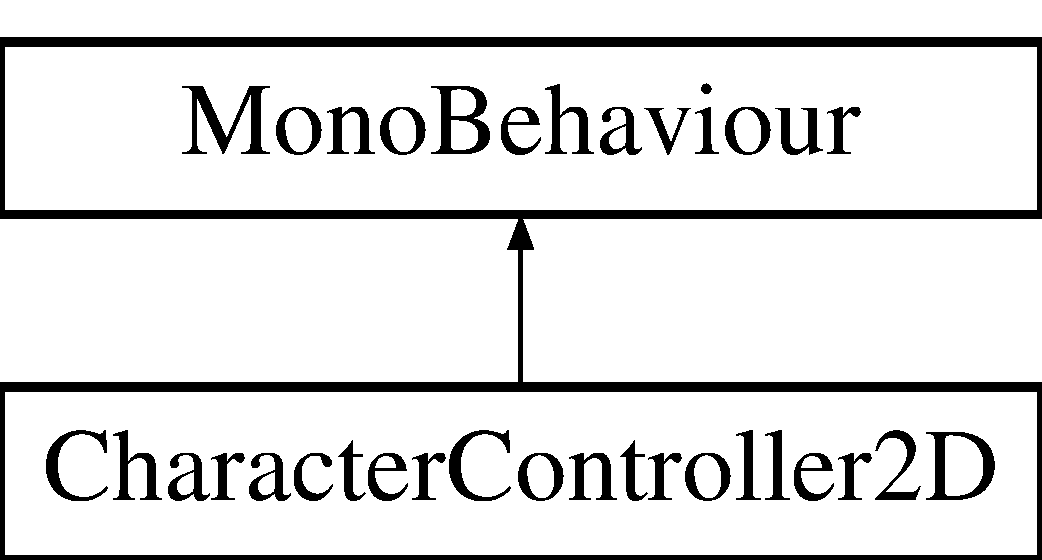
\includegraphics[height=2.000000cm]{class_character_controller2_d}
\end{center}
\end{figure}
\subsection*{Public Member Functions}
\begin{DoxyCompactItemize}
\item 
void \hyperlink{class_character_controller2_d_a63dec3eea904614ce11fff4d0b1f3374}{Awake} ()
\begin{DoxyCompactList}\small\item\em Inicjalizacja i ustawienie poczatkowych wartosci parametrow. \end{DoxyCompactList}\item 
void \hyperlink{class_character_controller2_d_adbd530fe94a846d57ed2c9f322491ab3}{Add\+Force} (Vector2 force)
\begin{DoxyCompactList}\small\item\em Dodanie dodatkowej predkosci. \end{DoxyCompactList}\item 
void \hyperlink{class_character_controller2_d_a5ed35a778ec714e5783d6f0570bca703}{Set\+Force} (Vector2 force)
\begin{DoxyCompactList}\small\item\em Ustawienie predkosci. \end{DoxyCompactList}\item 
void \hyperlink{class_character_controller2_d_a8fd797b25fef289cbc1993f94dfb9b48}{Set\+Horizontal\+Force} (float x)
\begin{DoxyCompactList}\small\item\em Ustawienie predkosci w poziomie. \end{DoxyCompactList}\item 
void \hyperlink{class_character_controller2_d_a29d14b0bb79f8661d9655ab9bed074e2}{Set\+Vertical\+Force} (float y)
\begin{DoxyCompactList}\small\item\em Ustawienie predkosci w pionie. \end{DoxyCompactList}\item 
void \hyperlink{class_character_controller2_d_aa42cc475784c2a2f5ca406669504824e}{Jump} ()
\begin{DoxyCompactList}\small\item\em Wykonanie skoku. \end{DoxyCompactList}\item 
void \hyperlink{class_character_controller2_d_aa16cb1f7b8c01f326f8b0b1508590dd7}{Late\+Update} ()
\begin{DoxyCompactList}\small\item\em Wykonywane po wywolaniu aktualizacji obiektow. Uwzglednienie wplywu czasu na czestotliwosc skokow i ruch, wplyw grawitacji na ruch w pionie. \end{DoxyCompactList}\item 
void \hyperlink{class_character_controller2_d_a9ac0f6a16c9a0e7190e5645a9ba77667}{On\+Trigger\+Enter2\+D} (Collider2\+D other)
\begin{DoxyCompactList}\small\item\em Wykrycie ze gracz znalazl sie w innym srodowisku (np. wodzie). \end{DoxyCompactList}\item 
void \hyperlink{class_character_controller2_d_a91e2f7eefc4b8e8590f8eca161d9a655}{On\+Trigger\+Exit2\+D} (Collider2\+D other)
\begin{DoxyCompactList}\small\item\em Wyjscie ze srodowiska o zmienionych parametrach. \end{DoxyCompactList}\end{DoxyCompactItemize}
\subsection*{Public Attributes}
\begin{DoxyCompactItemize}
\item 
Layer\+Mask \hyperlink{class_character_controller2_d_a239fc145e05e239c584bf7b1783b590e}{Platform\+Mask}
\begin{DoxyCompactList}\small\item\em Layer mask uzywany do wykrywania kolizji. Obiekty na tej warstwie uczestnicza w kolizji. \end{DoxyCompactList}\item 
\hyperlink{class_controller_parameters2_d}{Controller\+Parameters2\+D} \hyperlink{class_character_controller2_d_a33b6d08469389f16262f8a179ec3c873}{Default\+Parameters}
\begin{DoxyCompactList}\small\item\em Domyslne parametry kontrolera. \end{DoxyCompactList}\end{DoxyCompactItemize}
\subsection*{Properties}
\begin{DoxyCompactItemize}
\item 
\hyperlink{class_controller_state2_d}{Controller\+State2\+D} \hyperlink{class_character_controller2_d_a5e65ffc5d4f73920480727f2bf58e978}{State}\hspace{0.3cm}{\ttfamily  \mbox{[}get\mbox{]}}
\begin{DoxyCompactList}\small\item\em Stan gracza, informujacy o kolizjach w jakich bierze udzial. \end{DoxyCompactList}\item 
Vector2 \hyperlink{class_character_controller2_d_af48e21d4114c7f48f97fe924956b3d10}{Velocity}\hspace{0.3cm}{\ttfamily  \mbox{[}get\mbox{]}}
\begin{DoxyCompactList}\small\item\em Predkosc gracza. \end{DoxyCompactList}\item 
bool \hyperlink{class_character_controller2_d_aa693a23e691347cf526060141fad519e}{Handle\+Collisions}\hspace{0.3cm}{\ttfamily  \mbox{[}get, set\mbox{]}}
\begin{DoxyCompactList}\small\item\em Zmienna typu bool, mowiaca czy nalezy obsluzyc kolizje. \end{DoxyCompactList}\item 
\hyperlink{class_controller_parameters2_d}{Controller\+Parameters2\+D} \hyperlink{class_character_controller2_d_a408542bab9592c3d0d4ca432a5775ce6}{Parameters}\hspace{0.3cm}{\ttfamily  \mbox{[}get\mbox{]}}
\begin{DoxyCompactList}\small\item\em Zwraca nadpisane lub w przypadku braku nadpisania, domyslne parametry kontrolera. \end{DoxyCompactList}\item 
Game\+Object \hyperlink{class_character_controller2_d_ae2f301ab8f2d3b4290a2780d021e44fb}{Standing\+On}\hspace{0.3cm}{\ttfamily  \mbox{[}get\mbox{]}}
\begin{DoxyCompactList}\small\item\em Standing\+On \end{DoxyCompactList}\item 
Vector3 \hyperlink{class_character_controller2_d_a9eaf0dd583c426b16264c87a7d64d993}{Platform\+Velocity}\hspace{0.3cm}{\ttfamily  \mbox{[}get\mbox{]}}
\begin{DoxyCompactList}\small\item\em Predkosc platformy, na ktorej stoi gracz. \end{DoxyCompactList}\item 
bool \hyperlink{class_character_controller2_d_a79855579d0cbd33e1ed08df1c513bb0f}{Can\+Jump}\hspace{0.3cm}{\ttfamily  \mbox{[}get\mbox{]}}
\begin{DoxyCompactList}\small\item\em Sprawdza czy mozna wykonac skok zaleznie od ustawionej wartosci Jump\+Behavior. \end{DoxyCompactList}\end{DoxyCompactItemize}


\subsection{Detailed Description}
klasa \hyperlink{class_character_controller2_d}{Character\+Controller2\+D} 



\subsection{Member Function Documentation}
\hypertarget{class_character_controller2_d_adbd530fe94a846d57ed2c9f322491ab3}{}\index{Character\+Controller2\+D@{Character\+Controller2\+D}!Add\+Force@{Add\+Force}}
\index{Add\+Force@{Add\+Force}!Character\+Controller2\+D@{Character\+Controller2\+D}}
\subsubsection[{Add\+Force(\+Vector2 force)}]{\setlength{\rightskip}{0pt plus 5cm}void Character\+Controller2\+D.\+Add\+Force (
\begin{DoxyParamCaption}
\item[{Vector2}]{force}
\end{DoxyParamCaption}
)}\label{class_character_controller2_d_adbd530fe94a846d57ed2c9f322491ab3}


Dodanie dodatkowej predkosci. 

\hypertarget{class_character_controller2_d_a63dec3eea904614ce11fff4d0b1f3374}{}\index{Character\+Controller2\+D@{Character\+Controller2\+D}!Awake@{Awake}}
\index{Awake@{Awake}!Character\+Controller2\+D@{Character\+Controller2\+D}}
\subsubsection[{Awake()}]{\setlength{\rightskip}{0pt plus 5cm}void Character\+Controller2\+D.\+Awake (
\begin{DoxyParamCaption}
{}
\end{DoxyParamCaption}
)}\label{class_character_controller2_d_a63dec3eea904614ce11fff4d0b1f3374}


Inicjalizacja i ustawienie poczatkowych wartosci parametrow. 

Obliczenie rozmiarow boxu, ktory moze uczestniczyc w kolizjach z innymi brylami sztywnymi. Od wartosci odejmowane sa skiny, z ktorych wychodza promienie wykrywajace kolizje (skin to waska ramka wokol obiektu, istniejaca po wewnetrznej stronie obiektu, sluzaca do wykrywania kolizji). Nastepnie obliczane sa odstepy pomiedzy promieniami wykrywajacymi kolizje. \hypertarget{class_character_controller2_d_aa42cc475784c2a2f5ca406669504824e}{}\index{Character\+Controller2\+D@{Character\+Controller2\+D}!Jump@{Jump}}
\index{Jump@{Jump}!Character\+Controller2\+D@{Character\+Controller2\+D}}
\subsubsection[{Jump()}]{\setlength{\rightskip}{0pt plus 5cm}void Character\+Controller2\+D.\+Jump (
\begin{DoxyParamCaption}
{}
\end{DoxyParamCaption}
)}\label{class_character_controller2_d_aa42cc475784c2a2f5ca406669504824e}


Wykonanie skoku. 

\hypertarget{class_character_controller2_d_aa16cb1f7b8c01f326f8b0b1508590dd7}{}\index{Character\+Controller2\+D@{Character\+Controller2\+D}!Late\+Update@{Late\+Update}}
\index{Late\+Update@{Late\+Update}!Character\+Controller2\+D@{Character\+Controller2\+D}}
\subsubsection[{Late\+Update()}]{\setlength{\rightskip}{0pt plus 5cm}void Character\+Controller2\+D.\+Late\+Update (
\begin{DoxyParamCaption}
{}
\end{DoxyParamCaption}
)}\label{class_character_controller2_d_aa16cb1f7b8c01f326f8b0b1508590dd7}


Wykonywane po wywolaniu aktualizacji obiektow. Uwzglednienie wplywu czasu na czestotliwosc skokow i ruch, wplyw grawitacji na ruch w pionie. 

\hypertarget{class_character_controller2_d_a9ac0f6a16c9a0e7190e5645a9ba77667}{}\index{Character\+Controller2\+D@{Character\+Controller2\+D}!On\+Trigger\+Enter2\+D@{On\+Trigger\+Enter2\+D}}
\index{On\+Trigger\+Enter2\+D@{On\+Trigger\+Enter2\+D}!Character\+Controller2\+D@{Character\+Controller2\+D}}
\subsubsection[{On\+Trigger\+Enter2\+D(\+Collider2\+D other)}]{\setlength{\rightskip}{0pt plus 5cm}void Character\+Controller2\+D.\+On\+Trigger\+Enter2\+D (
\begin{DoxyParamCaption}
\item[{Collider2\+D}]{other}
\end{DoxyParamCaption}
)}\label{class_character_controller2_d_a9ac0f6a16c9a0e7190e5645a9ba77667}


Wykrycie ze gracz znalazl sie w innym srodowisku (np. wodzie). 

Nadpisanie parametrow kontrolera. \hypertarget{class_character_controller2_d_a91e2f7eefc4b8e8590f8eca161d9a655}{}\index{Character\+Controller2\+D@{Character\+Controller2\+D}!On\+Trigger\+Exit2\+D@{On\+Trigger\+Exit2\+D}}
\index{On\+Trigger\+Exit2\+D@{On\+Trigger\+Exit2\+D}!Character\+Controller2\+D@{Character\+Controller2\+D}}
\subsubsection[{On\+Trigger\+Exit2\+D(\+Collider2\+D other)}]{\setlength{\rightskip}{0pt plus 5cm}void Character\+Controller2\+D.\+On\+Trigger\+Exit2\+D (
\begin{DoxyParamCaption}
\item[{Collider2\+D}]{other}
\end{DoxyParamCaption}
)}\label{class_character_controller2_d_a91e2f7eefc4b8e8590f8eca161d9a655}


Wyjscie ze srodowiska o zmienionych parametrach. 

Parametry nie sa juz nadpisywane poprzednimi wartosciami. \hypertarget{class_character_controller2_d_a5ed35a778ec714e5783d6f0570bca703}{}\index{Character\+Controller2\+D@{Character\+Controller2\+D}!Set\+Force@{Set\+Force}}
\index{Set\+Force@{Set\+Force}!Character\+Controller2\+D@{Character\+Controller2\+D}}
\subsubsection[{Set\+Force(\+Vector2 force)}]{\setlength{\rightskip}{0pt plus 5cm}void Character\+Controller2\+D.\+Set\+Force (
\begin{DoxyParamCaption}
\item[{Vector2}]{force}
\end{DoxyParamCaption}
)}\label{class_character_controller2_d_a5ed35a778ec714e5783d6f0570bca703}


Ustawienie predkosci. 

\hypertarget{class_character_controller2_d_a8fd797b25fef289cbc1993f94dfb9b48}{}\index{Character\+Controller2\+D@{Character\+Controller2\+D}!Set\+Horizontal\+Force@{Set\+Horizontal\+Force}}
\index{Set\+Horizontal\+Force@{Set\+Horizontal\+Force}!Character\+Controller2\+D@{Character\+Controller2\+D}}
\subsubsection[{Set\+Horizontal\+Force(float x)}]{\setlength{\rightskip}{0pt plus 5cm}void Character\+Controller2\+D.\+Set\+Horizontal\+Force (
\begin{DoxyParamCaption}
\item[{float}]{x}
\end{DoxyParamCaption}
)}\label{class_character_controller2_d_a8fd797b25fef289cbc1993f94dfb9b48}


Ustawienie predkosci w poziomie. 

\hypertarget{class_character_controller2_d_a29d14b0bb79f8661d9655ab9bed074e2}{}\index{Character\+Controller2\+D@{Character\+Controller2\+D}!Set\+Vertical\+Force@{Set\+Vertical\+Force}}
\index{Set\+Vertical\+Force@{Set\+Vertical\+Force}!Character\+Controller2\+D@{Character\+Controller2\+D}}
\subsubsection[{Set\+Vertical\+Force(float y)}]{\setlength{\rightskip}{0pt plus 5cm}void Character\+Controller2\+D.\+Set\+Vertical\+Force (
\begin{DoxyParamCaption}
\item[{float}]{y}
\end{DoxyParamCaption}
)}\label{class_character_controller2_d_a29d14b0bb79f8661d9655ab9bed074e2}


Ustawienie predkosci w pionie. 



\subsection{Member Data Documentation}
\hypertarget{class_character_controller2_d_a33b6d08469389f16262f8a179ec3c873}{}\index{Character\+Controller2\+D@{Character\+Controller2\+D}!Default\+Parameters@{Default\+Parameters}}
\index{Default\+Parameters@{Default\+Parameters}!Character\+Controller2\+D@{Character\+Controller2\+D}}
\subsubsection[{Default\+Parameters}]{\setlength{\rightskip}{0pt plus 5cm}{\bf Controller\+Parameters2\+D} Character\+Controller2\+D.\+Default\+Parameters}\label{class_character_controller2_d_a33b6d08469389f16262f8a179ec3c873}


Domyslne parametry kontrolera. 

\hypertarget{class_character_controller2_d_a239fc145e05e239c584bf7b1783b590e}{}\index{Character\+Controller2\+D@{Character\+Controller2\+D}!Platform\+Mask@{Platform\+Mask}}
\index{Platform\+Mask@{Platform\+Mask}!Character\+Controller2\+D@{Character\+Controller2\+D}}
\subsubsection[{Platform\+Mask}]{\setlength{\rightskip}{0pt plus 5cm}Layer\+Mask Character\+Controller2\+D.\+Platform\+Mask}\label{class_character_controller2_d_a239fc145e05e239c584bf7b1783b590e}


Layer mask uzywany do wykrywania kolizji. Obiekty na tej warstwie uczestnicza w kolizji. 



\subsection{Property Documentation}
\hypertarget{class_character_controller2_d_a79855579d0cbd33e1ed08df1c513bb0f}{}\index{Character\+Controller2\+D@{Character\+Controller2\+D}!Can\+Jump@{Can\+Jump}}
\index{Can\+Jump@{Can\+Jump}!Character\+Controller2\+D@{Character\+Controller2\+D}}
\subsubsection[{Can\+Jump}]{\setlength{\rightskip}{0pt plus 5cm}bool Character\+Controller2\+D.\+Can\+Jump\hspace{0.3cm}{\ttfamily [get]}}\label{class_character_controller2_d_a79855579d0cbd33e1ed08df1c513bb0f}


Sprawdza czy mozna wykonac skok zaleznie od ustawionej wartosci Jump\+Behavior. 

\hypertarget{class_character_controller2_d_aa693a23e691347cf526060141fad519e}{}\index{Character\+Controller2\+D@{Character\+Controller2\+D}!Handle\+Collisions@{Handle\+Collisions}}
\index{Handle\+Collisions@{Handle\+Collisions}!Character\+Controller2\+D@{Character\+Controller2\+D}}
\subsubsection[{Handle\+Collisions}]{\setlength{\rightskip}{0pt plus 5cm}bool Character\+Controller2\+D.\+Handle\+Collisions\hspace{0.3cm}{\ttfamily [get]}, {\ttfamily [set]}}\label{class_character_controller2_d_aa693a23e691347cf526060141fad519e}


Zmienna typu bool, mowiaca czy nalezy obsluzyc kolizje. 

\hypertarget{class_character_controller2_d_a408542bab9592c3d0d4ca432a5775ce6}{}\index{Character\+Controller2\+D@{Character\+Controller2\+D}!Parameters@{Parameters}}
\index{Parameters@{Parameters}!Character\+Controller2\+D@{Character\+Controller2\+D}}
\subsubsection[{Parameters}]{\setlength{\rightskip}{0pt plus 5cm}{\bf Controller\+Parameters2\+D} Character\+Controller2\+D.\+Parameters\hspace{0.3cm}{\ttfamily [get]}}\label{class_character_controller2_d_a408542bab9592c3d0d4ca432a5775ce6}


Zwraca nadpisane lub w przypadku braku nadpisania, domyslne parametry kontrolera. 

\hypertarget{class_character_controller2_d_a9eaf0dd583c426b16264c87a7d64d993}{}\index{Character\+Controller2\+D@{Character\+Controller2\+D}!Platform\+Velocity@{Platform\+Velocity}}
\index{Platform\+Velocity@{Platform\+Velocity}!Character\+Controller2\+D@{Character\+Controller2\+D}}
\subsubsection[{Platform\+Velocity}]{\setlength{\rightskip}{0pt plus 5cm}Vector3 Character\+Controller2\+D.\+Platform\+Velocity\hspace{0.3cm}{\ttfamily [get]}}\label{class_character_controller2_d_a9eaf0dd583c426b16264c87a7d64d993}


Predkosc platformy, na ktorej stoi gracz. 

\hypertarget{class_character_controller2_d_ae2f301ab8f2d3b4290a2780d021e44fb}{}\index{Character\+Controller2\+D@{Character\+Controller2\+D}!Standing\+On@{Standing\+On}}
\index{Standing\+On@{Standing\+On}!Character\+Controller2\+D@{Character\+Controller2\+D}}
\subsubsection[{Standing\+On}]{\setlength{\rightskip}{0pt plus 5cm}Game\+Object Character\+Controller2\+D.\+Standing\+On\hspace{0.3cm}{\ttfamily [get]}}\label{class_character_controller2_d_ae2f301ab8f2d3b4290a2780d021e44fb}


Standing\+On 

\hypertarget{class_character_controller2_d_a5e65ffc5d4f73920480727f2bf58e978}{}\index{Character\+Controller2\+D@{Character\+Controller2\+D}!State@{State}}
\index{State@{State}!Character\+Controller2\+D@{Character\+Controller2\+D}}
\subsubsection[{State}]{\setlength{\rightskip}{0pt plus 5cm}{\bf Controller\+State2\+D} Character\+Controller2\+D.\+State\hspace{0.3cm}{\ttfamily [get]}}\label{class_character_controller2_d_a5e65ffc5d4f73920480727f2bf58e978}


Stan gracza, informujacy o kolizjach w jakich bierze udzial. 

\hypertarget{class_character_controller2_d_af48e21d4114c7f48f97fe924956b3d10}{}\index{Character\+Controller2\+D@{Character\+Controller2\+D}!Velocity@{Velocity}}
\index{Velocity@{Velocity}!Character\+Controller2\+D@{Character\+Controller2\+D}}
\subsubsection[{Velocity}]{\setlength{\rightskip}{0pt plus 5cm}Vector2 Character\+Controller2\+D.\+Velocity\hspace{0.3cm}{\ttfamily [get]}}\label{class_character_controller2_d_af48e21d4114c7f48f97fe924956b3d10}


Predkosc gracza. 



The documentation for this class was generated from the following file\+:\begin{DoxyCompactItemize}
\item 
C\+:/\+Users/\+Paul/\+Projects/\+Unity\+Game/\+Projekt/\+Assets/\+Code/Character\+Controller2\+D.\+cs\end{DoxyCompactItemize}

\hypertarget{class_controller_parameters2_d}{}\section{Controller\+Parameters2\+D Class Reference}
\label{class_controller_parameters2_d}\index{Controller\+Parameters2\+D@{Controller\+Parameters2\+D}}


klasa \hyperlink{class_controller_parameters2_d}{Controller\+Parameters2\+D}  


\subsection*{Public Types}
\begin{DoxyCompactItemize}
\item 
\hypertarget{class_controller_parameters2_d_a2838d319f4380bc1120750fdff3dd22f}{}enum \hyperlink{class_controller_parameters2_d_a2838d319f4380bc1120750fdff3dd22f}{Jump\+Behavior} \{ {\bfseries Can\+Jump\+On\+Ground}, 
{\bfseries Can\+Jump\+Anywhere}, 
{\bfseries Cant\+Jump}
 \}\label{class_controller_parameters2_d_a2838d319f4380bc1120750fdff3dd22f}
\begin{DoxyCompactList}\small\item\em Czy mozna wykonac skok i w jakich okolicznosciach. \end{DoxyCompactList}
\end{DoxyCompactItemize}
\subsection*{Public Attributes}
\begin{DoxyCompactItemize}
\item 
\hypertarget{class_controller_parameters2_d_a06ebe9f5ed4fb8a39c1ed11f36659b2b}{}Vector2 \hyperlink{class_controller_parameters2_d_a06ebe9f5ed4fb8a39c1ed11f36659b2b}{Max\+Velocity} = new Vector2(float.\+Max\+Value, float.\+Max\+Value)\label{class_controller_parameters2_d_a06ebe9f5ed4fb8a39c1ed11f36659b2b}

\begin{DoxyCompactList}\small\item\em Ustawienie maksymalnej predkosci gracza. \end{DoxyCompactList}\item 
float \hyperlink{class_controller_parameters2_d_ae706235bff2d67da0d71293bef2ea8d1}{Slope\+Limit} = 30
\begin{DoxyCompactList}\small\item\em Slope\+Limit. \end{DoxyCompactList}\item 
\hypertarget{class_controller_parameters2_d_ae83e87db83f426c232a43dd15e30fb38}{}float \hyperlink{class_controller_parameters2_d_ae83e87db83f426c232a43dd15e30fb38}{Gravity} = -\/25f\label{class_controller_parameters2_d_ae83e87db83f426c232a43dd15e30fb38}

\begin{DoxyCompactList}\small\item\em Grawitacja. \end{DoxyCompactList}\item 
\hypertarget{class_controller_parameters2_d_aa709ad9bce9649d1fbb6e5146c141325}{}\hyperlink{class_controller_parameters2_d_a2838d319f4380bc1120750fdff3dd22f}{Jump\+Behavior} \hyperlink{class_controller_parameters2_d_aa709ad9bce9649d1fbb6e5146c141325}{Jump\+Restrictions}\label{class_controller_parameters2_d_aa709ad9bce9649d1fbb6e5146c141325}

\begin{DoxyCompactList}\small\item\em Jump\+Restrictions. \end{DoxyCompactList}\item 
\hypertarget{class_controller_parameters2_d_ac1215bef2bee5c3e555b92e79ad447cb}{}float \hyperlink{class_controller_parameters2_d_ac1215bef2bee5c3e555b92e79ad447cb}{Jump\+Frequency} = .\+25f\label{class_controller_parameters2_d_ac1215bef2bee5c3e555b92e79ad447cb}

\begin{DoxyCompactList}\small\item\em Częstotliwość skoku. \end{DoxyCompactList}\item 
\hypertarget{class_controller_parameters2_d_ae92dcce1c474adc687bcfa45ca02ae27}{}float \hyperlink{class_controller_parameters2_d_ae92dcce1c474adc687bcfa45ca02ae27}{Jump\+Magnitude} = 12\label{class_controller_parameters2_d_ae92dcce1c474adc687bcfa45ca02ae27}

\begin{DoxyCompactList}\small\item\em Siła skoku. \end{DoxyCompactList}\end{DoxyCompactItemize}


\subsection{Detailed Description}
klasa \hyperlink{class_controller_parameters2_d}{Controller\+Parameters2\+D} 



\subsection{Member Data Documentation}
\hypertarget{class_controller_parameters2_d_ae706235bff2d67da0d71293bef2ea8d1}{}\index{Controller\+Parameters2\+D@{Controller\+Parameters2\+D}!Slope\+Limit@{Slope\+Limit}}
\index{Slope\+Limit@{Slope\+Limit}!Controller\+Parameters2\+D@{Controller\+Parameters2\+D}}
\subsubsection[{Slope\+Limit}]{\setlength{\rightskip}{0pt plus 5cm}float Controller\+Parameters2\+D.\+Slope\+Limit = 30}\label{class_controller_parameters2_d_ae706235bff2d67da0d71293bef2ea8d1}


Slope\+Limit. 

Nie mozna wejsc na teren o nachyleniu wiekszym od 30 stopni. Ustalenie grawitacji, dopusczalnej czestotliwosci skokow i ich sily. 

The documentation for this class was generated from the following file\+:\begin{DoxyCompactItemize}
\item 
C\+:/\+Users/\+Paul/\+Projects/\+Unity\+Game/\+Projekt/\+Assets/\+Code/Controller\+Parameters2\+D.\+cs\end{DoxyCompactItemize}

\hypertarget{class_controller_physics_volume2_d}{}\section{Controller\+Physics\+Volume2\+D Class Reference}
\label{class_controller_physics_volume2_d}\index{Controller\+Physics\+Volume2\+D@{Controller\+Physics\+Volume2\+D}}


klasa \hyperlink{class_controller_physics_volume2_d}{Controller\+Physics\+Volume2\+D}  


Inheritance diagram for Controller\+Physics\+Volume2\+D\+:\begin{figure}[H]
\begin{center}
\leavevmode
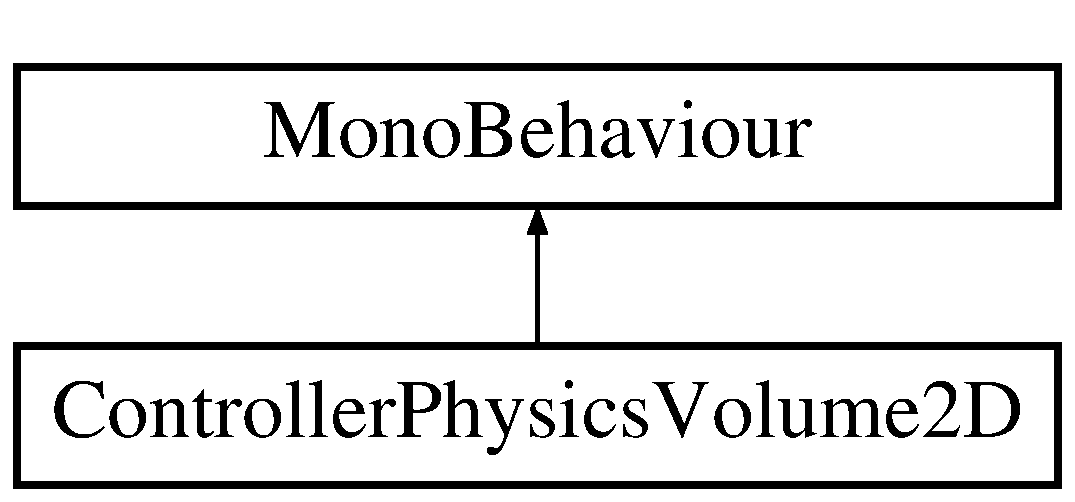
\includegraphics[height=2.000000cm]{class_controller_physics_volume2_d}
\end{center}
\end{figure}
\subsection*{Public Attributes}
\begin{DoxyCompactItemize}
\item 
\hyperlink{class_controller_parameters2_d}{Controller\+Parameters2\+D} \hyperlink{class_controller_physics_volume2_d_a57a01a60fe2b7a3ab0bd7808211a42b7}{Parameters}
\begin{DoxyCompactList}\small\item\em Uzywane przy zmianie srodowiska w jakim jest gracz (np. na wode), co wplywa na parametry kontrolera. \end{DoxyCompactList}\end{DoxyCompactItemize}


\subsection{Detailed Description}
klasa \hyperlink{class_controller_physics_volume2_d}{Controller\+Physics\+Volume2\+D} 



\subsection{Member Data Documentation}
\hypertarget{class_controller_physics_volume2_d_a57a01a60fe2b7a3ab0bd7808211a42b7}{}\index{Controller\+Physics\+Volume2\+D@{Controller\+Physics\+Volume2\+D}!Parameters@{Parameters}}
\index{Parameters@{Parameters}!Controller\+Physics\+Volume2\+D@{Controller\+Physics\+Volume2\+D}}
\subsubsection[{Parameters}]{\setlength{\rightskip}{0pt plus 5cm}{\bf Controller\+Parameters2\+D} Controller\+Physics\+Volume2\+D.\+Parameters}\label{class_controller_physics_volume2_d_a57a01a60fe2b7a3ab0bd7808211a42b7}


Uzywane przy zmianie srodowiska w jakim jest gracz (np. na wode), co wplywa na parametry kontrolera. 



The documentation for this class was generated from the following file\+:\begin{DoxyCompactItemize}
\item 
C\+:/\+Users/\+Paul/\+Projects/\+Unity\+Game/\+Projekt/\+Assets/\+Code/Controller\+Physics\+Volume2\+D.\+cs\end{DoxyCompactItemize}

\hypertarget{class_controller_state2_d}{}\section{Controller\+State2\+D Class Reference}
\label{class_controller_state2_d}\index{Controller\+State2\+D@{Controller\+State2\+D}}


klasa \hyperlink{class_controller_state2_d}{Controller\+State2\+D}  


\subsection*{Public Member Functions}
\begin{DoxyCompactItemize}
\item 
void \hyperlink{class_controller_state2_d_a227682256d3eabc548dcd982cbcb7aef}{Reset} ()
\begin{DoxyCompactList}\small\item\em Reset stanu \end{DoxyCompactList}\item 
override string \hyperlink{class_controller_state2_d_af8f1803156a41e5a8ca0c7c6a7f12865}{To\+String} ()
\begin{DoxyCompactList}\small\item\em Debug \end{DoxyCompactList}\end{DoxyCompactItemize}
\subsection*{Properties}
\begin{DoxyCompactItemize}
\item 
bool \hyperlink{class_controller_state2_d_ab415da9f261852bca7ba1ec57adf41bb}{Is\+Colliding\+Right}\hspace{0.3cm}{\ttfamily  \mbox{[}get, set\mbox{]}}
\begin{DoxyCompactList}\small\item\em Kolizja z prawej strony \end{DoxyCompactList}\item 
bool \hyperlink{class_controller_state2_d_a4774afc53858b57f6016e1fb620268c4}{Is\+Colliding\+Left}\hspace{0.3cm}{\ttfamily  \mbox{[}get, set\mbox{]}}
\begin{DoxyCompactList}\small\item\em Kolizja z lewej strony \end{DoxyCompactList}\item 
bool \hyperlink{class_controller_state2_d_a31e26c803a9fa52216eccaf2adb94b67}{Is\+Colliding\+Above}\hspace{0.3cm}{\ttfamily  \mbox{[}get, set\mbox{]}}
\begin{DoxyCompactList}\small\item\em Kolizja powyżej \end{DoxyCompactList}\item 
bool \hyperlink{class_controller_state2_d_ac23ed207ad3b8225b8cdea0505165c8a}{Is\+Colliding\+Below}\hspace{0.3cm}{\ttfamily  \mbox{[}get, set\mbox{]}}
\begin{DoxyCompactList}\small\item\em Kolizja z poniżej \end{DoxyCompactList}\item 
bool \hyperlink{class_controller_state2_d_a813f7c0a080a2b3f784751bb4fa63057}{Is\+Moving\+Down\+Slope}\hspace{0.3cm}{\ttfamily  \mbox{[}get, set\mbox{]}}
\begin{DoxyCompactList}\small\item\em Kolizja ruch po pochyłej (dół) \end{DoxyCompactList}\item 
bool \hyperlink{class_controller_state2_d_ace3f85ee5879533e319143ee09b16f91}{Is\+Moving\+Up\+Slope}\hspace{0.3cm}{\ttfamily  \mbox{[}get, set\mbox{]}}
\begin{DoxyCompactList}\small\item\em Kolizja ruch po pochyłej (góra) \end{DoxyCompactList}\item 
bool \hyperlink{class_controller_state2_d_a895b129b6c8f95dd3aef68d9342a14d8}{Is\+Grounded}\hspace{0.3cm}{\ttfamily  \mbox{[}get\mbox{]}}
\begin{DoxyCompactList}\small\item\em Kolizja ziemia \end{DoxyCompactList}\item 
float \hyperlink{class_controller_state2_d_a724ea7c59fdf1d3c6f1e8fa80998651a}{Slope\+Angle}\hspace{0.3cm}{\ttfamily  \mbox{[}get, set\mbox{]}}
\begin{DoxyCompactList}\small\item\em Kąt pochyłej \end{DoxyCompactList}\item 
bool \hyperlink{class_controller_state2_d_a81b74ffe89ca998f186dfcc01cd74a80}{Has\+Collisions}\hspace{0.3cm}{\ttfamily  \mbox{[}get\mbox{]}}
\begin{DoxyCompactList}\small\item\em Kolizja jakakolwiek \end{DoxyCompactList}\end{DoxyCompactItemize}


\subsection{Detailed Description}
klasa \hyperlink{class_controller_state2_d}{Controller\+State2\+D} 



\subsection{Member Function Documentation}
\hypertarget{class_controller_state2_d_a227682256d3eabc548dcd982cbcb7aef}{}\index{Controller\+State2\+D@{Controller\+State2\+D}!Reset@{Reset}}
\index{Reset@{Reset}!Controller\+State2\+D@{Controller\+State2\+D}}
\subsubsection[{Reset()}]{\setlength{\rightskip}{0pt plus 5cm}void Controller\+State2\+D.\+Reset (
\begin{DoxyParamCaption}
{}
\end{DoxyParamCaption}
)}\label{class_controller_state2_d_a227682256d3eabc548dcd982cbcb7aef}


Reset stanu 

\hypertarget{class_controller_state2_d_af8f1803156a41e5a8ca0c7c6a7f12865}{}\index{Controller\+State2\+D@{Controller\+State2\+D}!To\+String@{To\+String}}
\index{To\+String@{To\+String}!Controller\+State2\+D@{Controller\+State2\+D}}
\subsubsection[{To\+String()}]{\setlength{\rightskip}{0pt plus 5cm}override string Controller\+State2\+D.\+To\+String (
\begin{DoxyParamCaption}
{}
\end{DoxyParamCaption}
)}\label{class_controller_state2_d_af8f1803156a41e5a8ca0c7c6a7f12865}


Debug 



\subsection{Property Documentation}
\hypertarget{class_controller_state2_d_a81b74ffe89ca998f186dfcc01cd74a80}{}\index{Controller\+State2\+D@{Controller\+State2\+D}!Has\+Collisions@{Has\+Collisions}}
\index{Has\+Collisions@{Has\+Collisions}!Controller\+State2\+D@{Controller\+State2\+D}}
\subsubsection[{Has\+Collisions}]{\setlength{\rightskip}{0pt plus 5cm}bool Controller\+State2\+D.\+Has\+Collisions\hspace{0.3cm}{\ttfamily [get]}}\label{class_controller_state2_d_a81b74ffe89ca998f186dfcc01cd74a80}


Kolizja jakakolwiek 

\hypertarget{class_controller_state2_d_a31e26c803a9fa52216eccaf2adb94b67}{}\index{Controller\+State2\+D@{Controller\+State2\+D}!Is\+Colliding\+Above@{Is\+Colliding\+Above}}
\index{Is\+Colliding\+Above@{Is\+Colliding\+Above}!Controller\+State2\+D@{Controller\+State2\+D}}
\subsubsection[{Is\+Colliding\+Above}]{\setlength{\rightskip}{0pt plus 5cm}bool Controller\+State2\+D.\+Is\+Colliding\+Above\hspace{0.3cm}{\ttfamily [get]}, {\ttfamily [set]}}\label{class_controller_state2_d_a31e26c803a9fa52216eccaf2adb94b67}


Kolizja powyżej 

\hypertarget{class_controller_state2_d_ac23ed207ad3b8225b8cdea0505165c8a}{}\index{Controller\+State2\+D@{Controller\+State2\+D}!Is\+Colliding\+Below@{Is\+Colliding\+Below}}
\index{Is\+Colliding\+Below@{Is\+Colliding\+Below}!Controller\+State2\+D@{Controller\+State2\+D}}
\subsubsection[{Is\+Colliding\+Below}]{\setlength{\rightskip}{0pt plus 5cm}bool Controller\+State2\+D.\+Is\+Colliding\+Below\hspace{0.3cm}{\ttfamily [get]}, {\ttfamily [set]}}\label{class_controller_state2_d_ac23ed207ad3b8225b8cdea0505165c8a}


Kolizja z poniżej 

\hypertarget{class_controller_state2_d_a4774afc53858b57f6016e1fb620268c4}{}\index{Controller\+State2\+D@{Controller\+State2\+D}!Is\+Colliding\+Left@{Is\+Colliding\+Left}}
\index{Is\+Colliding\+Left@{Is\+Colliding\+Left}!Controller\+State2\+D@{Controller\+State2\+D}}
\subsubsection[{Is\+Colliding\+Left}]{\setlength{\rightskip}{0pt plus 5cm}bool Controller\+State2\+D.\+Is\+Colliding\+Left\hspace{0.3cm}{\ttfamily [get]}, {\ttfamily [set]}}\label{class_controller_state2_d_a4774afc53858b57f6016e1fb620268c4}


Kolizja z lewej strony 

\hypertarget{class_controller_state2_d_ab415da9f261852bca7ba1ec57adf41bb}{}\index{Controller\+State2\+D@{Controller\+State2\+D}!Is\+Colliding\+Right@{Is\+Colliding\+Right}}
\index{Is\+Colliding\+Right@{Is\+Colliding\+Right}!Controller\+State2\+D@{Controller\+State2\+D}}
\subsubsection[{Is\+Colliding\+Right}]{\setlength{\rightskip}{0pt plus 5cm}bool Controller\+State2\+D.\+Is\+Colliding\+Right\hspace{0.3cm}{\ttfamily [get]}, {\ttfamily [set]}}\label{class_controller_state2_d_ab415da9f261852bca7ba1ec57adf41bb}


Kolizja z prawej strony 

\hypertarget{class_controller_state2_d_a895b129b6c8f95dd3aef68d9342a14d8}{}\index{Controller\+State2\+D@{Controller\+State2\+D}!Is\+Grounded@{Is\+Grounded}}
\index{Is\+Grounded@{Is\+Grounded}!Controller\+State2\+D@{Controller\+State2\+D}}
\subsubsection[{Is\+Grounded}]{\setlength{\rightskip}{0pt plus 5cm}bool Controller\+State2\+D.\+Is\+Grounded\hspace{0.3cm}{\ttfamily [get]}}\label{class_controller_state2_d_a895b129b6c8f95dd3aef68d9342a14d8}


Kolizja ziemia 

\hypertarget{class_controller_state2_d_a813f7c0a080a2b3f784751bb4fa63057}{}\index{Controller\+State2\+D@{Controller\+State2\+D}!Is\+Moving\+Down\+Slope@{Is\+Moving\+Down\+Slope}}
\index{Is\+Moving\+Down\+Slope@{Is\+Moving\+Down\+Slope}!Controller\+State2\+D@{Controller\+State2\+D}}
\subsubsection[{Is\+Moving\+Down\+Slope}]{\setlength{\rightskip}{0pt plus 5cm}bool Controller\+State2\+D.\+Is\+Moving\+Down\+Slope\hspace{0.3cm}{\ttfamily [get]}, {\ttfamily [set]}}\label{class_controller_state2_d_a813f7c0a080a2b3f784751bb4fa63057}


Kolizja ruch po pochyłej (dół) 

\hypertarget{class_controller_state2_d_ace3f85ee5879533e319143ee09b16f91}{}\index{Controller\+State2\+D@{Controller\+State2\+D}!Is\+Moving\+Up\+Slope@{Is\+Moving\+Up\+Slope}}
\index{Is\+Moving\+Up\+Slope@{Is\+Moving\+Up\+Slope}!Controller\+State2\+D@{Controller\+State2\+D}}
\subsubsection[{Is\+Moving\+Up\+Slope}]{\setlength{\rightskip}{0pt plus 5cm}bool Controller\+State2\+D.\+Is\+Moving\+Up\+Slope\hspace{0.3cm}{\ttfamily [get]}, {\ttfamily [set]}}\label{class_controller_state2_d_ace3f85ee5879533e319143ee09b16f91}


Kolizja ruch po pochyłej (góra) 

\hypertarget{class_controller_state2_d_a724ea7c59fdf1d3c6f1e8fa80998651a}{}\index{Controller\+State2\+D@{Controller\+State2\+D}!Slope\+Angle@{Slope\+Angle}}
\index{Slope\+Angle@{Slope\+Angle}!Controller\+State2\+D@{Controller\+State2\+D}}
\subsubsection[{Slope\+Angle}]{\setlength{\rightskip}{0pt plus 5cm}float Controller\+State2\+D.\+Slope\+Angle\hspace{0.3cm}{\ttfamily [get]}, {\ttfamily [set]}}\label{class_controller_state2_d_a724ea7c59fdf1d3c6f1e8fa80998651a}


Kąt pochyłej 



The documentation for this class was generated from the following file\+:\begin{DoxyCompactItemize}
\item 
C\+:/\+Users/\+Paul/\+Projects/\+Unity\+Game/\+Projekt/\+Assets/\+Code/Controller\+State2\+D.\+cs\end{DoxyCompactItemize}

\hypertarget{class_follow_path}{}\section{Follow\+Path Class Reference}
\label{class_follow_path}\index{Follow\+Path@{Follow\+Path}}


klasa \hyperlink{class_follow_path}{Follow\+Path}  


Inheritance diagram for Follow\+Path\+:\begin{figure}[H]
\begin{center}
\leavevmode
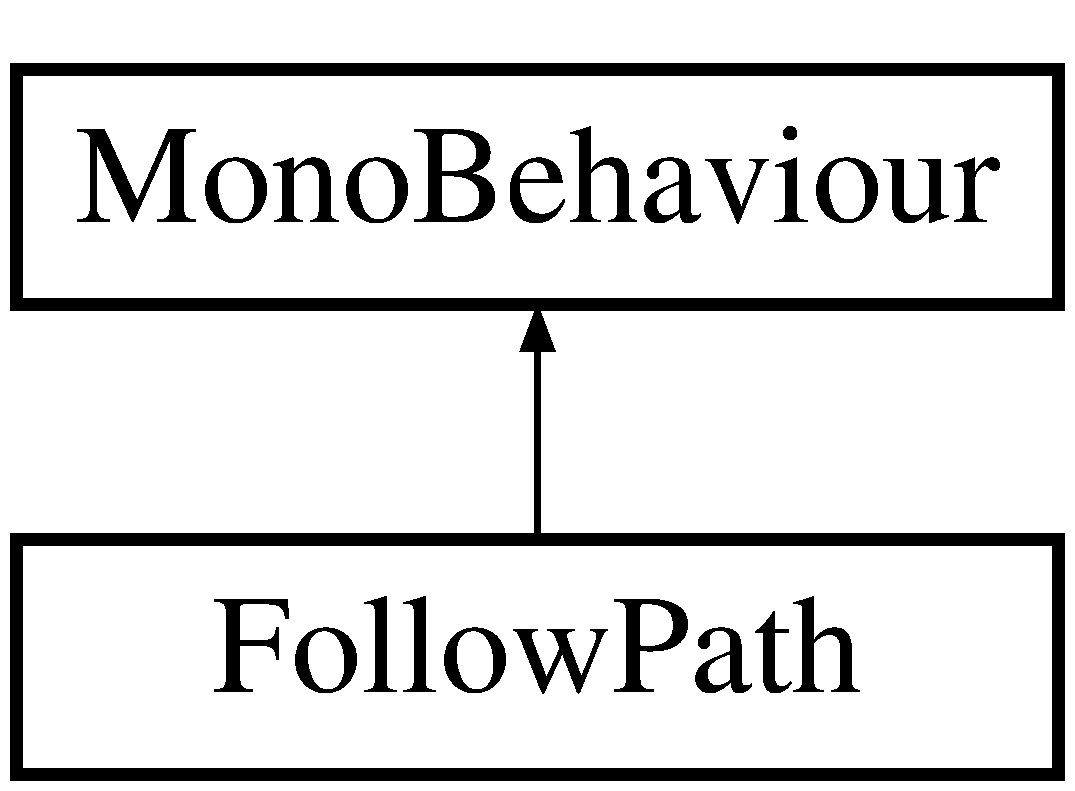
\includegraphics[height=2.000000cm]{class_follow_path}
\end{center}
\end{figure}
\subsection*{Public Types}
\begin{DoxyCompactItemize}
\item 
\hypertarget{class_follow_path_aa15222ed17c7bb53f199e5cb5e5c9cef}{}enum \hyperlink{class_follow_path_aa15222ed17c7bb53f199e5cb5e5c9cef}{Follow\+Type} \{ {\bfseries Move\+Towards}, 
{\bfseries Lerp}
 \}\label{class_follow_path_aa15222ed17c7bb53f199e5cb5e5c9cef}
\begin{DoxyCompactList}\small\item\em Wybor trybu ruchu. Lerp -\/ wykorzystujacy interpolacje liniowa. \end{DoxyCompactList}
\end{DoxyCompactItemize}
\subsection*{Public Member Functions}
\begin{DoxyCompactItemize}
\item 
\hypertarget{class_follow_path_a5e1828cf1cf7744c062a58e4a0d29605}{}void \hyperlink{class_follow_path_a5e1828cf1cf7744c062a58e4a0d29605}{Start} ()\label{class_follow_path_a5e1828cf1cf7744c062a58e4a0d29605}

\begin{DoxyCompactList}\small\item\em Inicjalizacja. \end{DoxyCompactList}\item 
void \hyperlink{class_follow_path_a157ad1da8560085de3542e46050d7183}{Update} ()
\end{DoxyCompactItemize}
\subsection*{Public Attributes}
\begin{DoxyCompactItemize}
\item 
\hypertarget{class_follow_path_a923cc736d703c012d1b6d8874291fa35}{}\hyperlink{class_follow_path_aa15222ed17c7bb53f199e5cb5e5c9cef}{Follow\+Type} \hyperlink{class_follow_path_a923cc736d703c012d1b6d8874291fa35}{Type} = Follow\+Type.\+Move\+Towards\label{class_follow_path_a923cc736d703c012d1b6d8874291fa35}

\begin{DoxyCompactList}\small\item\em Typ. \end{DoxyCompactList}\item 
\hypertarget{class_follow_path_a14f4aab3adc712c07ae9a02b87ffb2e3}{}\hyperlink{class_path_definition}{Path\+Definition} \hyperlink{class_follow_path_a14f4aab3adc712c07ae9a02b87ffb2e3}{Path}\label{class_follow_path_a14f4aab3adc712c07ae9a02b87ffb2e3}

\begin{DoxyCompactList}\small\item\em Ścieżka. \end{DoxyCompactList}\item 
\hypertarget{class_follow_path_a366b7ad38c7db477e1217ae5c364ac2b}{}float \hyperlink{class_follow_path_a366b7ad38c7db477e1217ae5c364ac2b}{Speed} = 1\label{class_follow_path_a366b7ad38c7db477e1217ae5c364ac2b}

\begin{DoxyCompactList}\small\item\em Prękość \end{DoxyCompactList}\item 
\hypertarget{class_follow_path_a7fd1ef16a8e77196e526d285197ed847}{}float \hyperlink{class_follow_path_a7fd1ef16a8e77196e526d285197ed847}{Max\+Distance\+To\+Goal} = .\+1f\label{class_follow_path_a7fd1ef16a8e77196e526d285197ed847}

\begin{DoxyCompactList}\small\item\em Maksymalna odległość \end{DoxyCompactList}\end{DoxyCompactItemize}


\subsection{Detailed Description}
klasa \hyperlink{class_follow_path}{Follow\+Path} 



\subsection{Member Function Documentation}
\hypertarget{class_follow_path_a157ad1da8560085de3542e46050d7183}{}\index{Follow\+Path@{Follow\+Path}!Update@{Update}}
\index{Update@{Update}!Follow\+Path@{Follow\+Path}}
\subsubsection[{Update()}]{\setlength{\rightskip}{0pt plus 5cm}void Follow\+Path.\+Update (
\begin{DoxyParamCaption}
{}
\end{DoxyParamCaption}
)}\label{class_follow_path_a157ad1da8560085de3542e46050d7183}
Obiekt stworzony bez sciezki, albo ze sciezka ktora nie ma co najmniej jednego punktu.

Argumenty\+: obecna pozycja, pozycja docelowa, predkosc (skalowana przez delta\+Time, aby zapewnic plynnosc animacji).

Sprawdzenie czy osiagnelismy cel i mozemy przemiescic sie do kolejnego punktu. 

The documentation for this class was generated from the following file\+:\begin{DoxyCompactItemize}
\item 
C\+:/\+Users/\+Paul/\+Projects/\+Unity\+Game/\+Projekt/\+Assets/\+Code/Follow\+Path.\+cs\end{DoxyCompactItemize}

\hypertarget{class_jump_platform}{}\section{Jump\+Platform Class Reference}
\label{class_jump_platform}\index{Jump\+Platform@{Jump\+Platform}}


klasa \hyperlink{class_jump_platform}{Jump\+Platform}  


Inheritance diagram for Jump\+Platform\+:\begin{figure}[H]
\begin{center}
\leavevmode
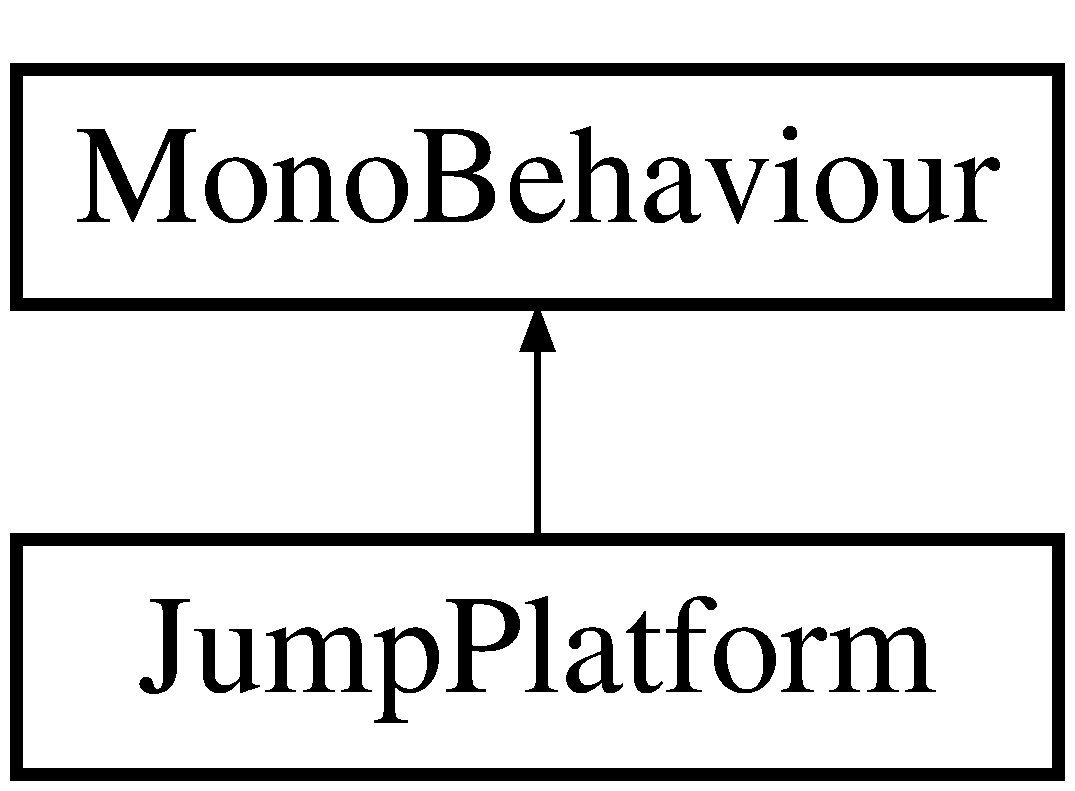
\includegraphics[height=2.000000cm]{class_jump_platform}
\end{center}
\end{figure}
\subsection*{Public Member Functions}
\begin{DoxyCompactItemize}
\item 
\hypertarget{class_jump_platform_ad1e3b06d092b641e4ef9e773aba1de6d}{}void \hyperlink{class_jump_platform_ad1e3b06d092b641e4ef9e773aba1de6d}{Controller\+Enter2\+D} (\hyperlink{class_character_controller2_d}{Character\+Controller2\+D} controller)\label{class_jump_platform_ad1e3b06d092b641e4ef9e773aba1de6d}

\begin{DoxyCompactList}\small\item\em Ustalenie Jump\+Magnitude. \end{DoxyCompactList}\end{DoxyCompactItemize}
\subsection*{Public Attributes}
\begin{DoxyCompactItemize}
\item 
\hypertarget{class_jump_platform_a089d1fb7693297d093994570c338ad75}{}float \hyperlink{class_jump_platform_a089d1fb7693297d093994570c338ad75}{Jump\+Magnitude} = 20\label{class_jump_platform_a089d1fb7693297d093994570c338ad75}

\begin{DoxyCompactList}\small\item\em Ustalenie sily skoku. \end{DoxyCompactList}\end{DoxyCompactItemize}


\subsection{Detailed Description}
klasa \hyperlink{class_jump_platform}{Jump\+Platform} 



The documentation for this class was generated from the following file\+:\begin{DoxyCompactItemize}
\item 
C\+:/\+Users/\+Paul/\+Projects/\+Unity\+Game/\+Projekt/\+Assets/\+Code/Jump\+Platform.\+cs\end{DoxyCompactItemize}

\hypertarget{class_path_definition}{}\section{Path\+Definition Class Reference}
\label{class_path_definition}\index{Path\+Definition@{Path\+Definition}}


klasa \hyperlink{class_path_definition}{Path\+Definition}  


Inheritance diagram for Path\+Definition\+:\begin{figure}[H]
\begin{center}
\leavevmode
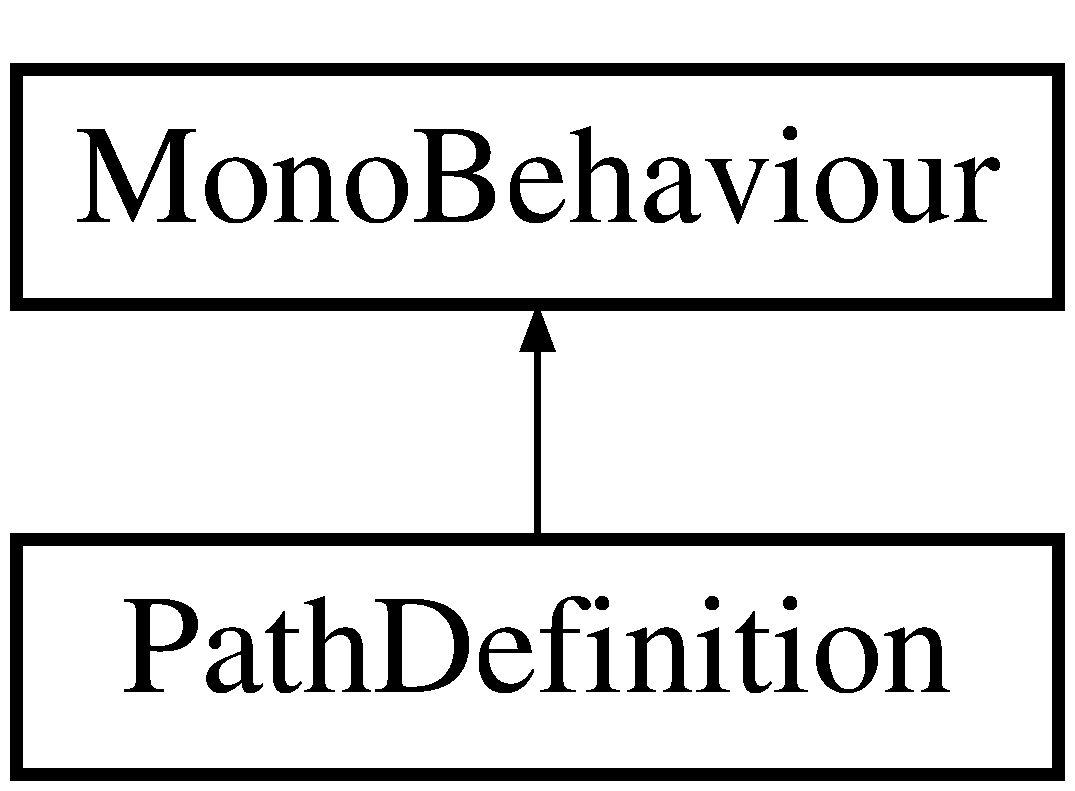
\includegraphics[height=2.000000cm]{class_path_definition}
\end{center}
\end{figure}
\subsection*{Public Member Functions}
\begin{DoxyCompactItemize}
\item 
I\+Enumerator$<$ Transform $>$ \hyperlink{class_path_definition_a0526b4b4e15883dad98b64bbed920f96}{Get\+Path\+Enumerator} ()
\item 
void \hyperlink{class_path_definition_a5539d857e10ad2827afc1fbce1512e47}{On\+Draw\+Gizmos} ()
\end{DoxyCompactItemize}
\subsection*{Public Attributes}
\begin{DoxyCompactItemize}
\item 
\hypertarget{class_path_definition_ab2d82757e323cdfcdb25cf2111c12310}{}Transform\mbox{[}$\,$\mbox{]} \hyperlink{class_path_definition_ab2d82757e323cdfcdb25cf2111c12310}{Points}\label{class_path_definition_ab2d82757e323cdfcdb25cf2111c12310}

\begin{DoxyCompactList}\small\item\em Punkty sciezki. \end{DoxyCompactList}\end{DoxyCompactItemize}


\subsection{Detailed Description}
klasa \hyperlink{class_path_definition}{Path\+Definition} 



\subsection{Member Function Documentation}
\hypertarget{class_path_definition_a0526b4b4e15883dad98b64bbed920f96}{}\index{Path\+Definition@{Path\+Definition}!Get\+Path\+Enumerator@{Get\+Path\+Enumerator}}
\index{Get\+Path\+Enumerator@{Get\+Path\+Enumerator}!Path\+Definition@{Path\+Definition}}
\subsubsection[{Get\+Path\+Enumerator()}]{\setlength{\rightskip}{0pt plus 5cm}I\+Enumerator$<$Transform$>$ Path\+Definition.\+Get\+Path\+Enumerator (
\begin{DoxyParamCaption}
{}
\end{DoxyParamCaption}
)}\label{class_path_definition_a0526b4b4e15883dad98b64bbed920f96}
Enumerator punktow w sciezce. Zapewnia poruszanie sie np. platform w obie strony po sciezce. \hypertarget{class_path_definition_a5539d857e10ad2827afc1fbce1512e47}{}\index{Path\+Definition@{Path\+Definition}!On\+Draw\+Gizmos@{On\+Draw\+Gizmos}}
\index{On\+Draw\+Gizmos@{On\+Draw\+Gizmos}!Path\+Definition@{Path\+Definition}}
\subsubsection[{On\+Draw\+Gizmos()}]{\setlength{\rightskip}{0pt plus 5cm}void Path\+Definition.\+On\+Draw\+Gizmos (
\begin{DoxyParamCaption}
{}
\end{DoxyParamCaption}
)}\label{class_path_definition_a5539d857e10ad2827afc1fbce1512e47}
Rysowanie linii miedzy punktami sciezki w Scene view, upewniajac sie czy istnieje odpowiednia ilosc punktow i omijajac usuniete. 

The documentation for this class was generated from the following file\+:\begin{DoxyCompactItemize}
\item 
C\+:/\+Users/\+Paul/\+Projects/\+Unity\+Game/\+Projekt/\+Assets/\+Code/Path\+Definition.\+cs\end{DoxyCompactItemize}

\hypertarget{class_player}{}\section{Player Class Reference}
\label{class_player}\index{Player@{Player}}


klasa \hyperlink{class_player}{Player}  


Inheritance diagram for Player\+:\begin{figure}[H]
\begin{center}
\leavevmode
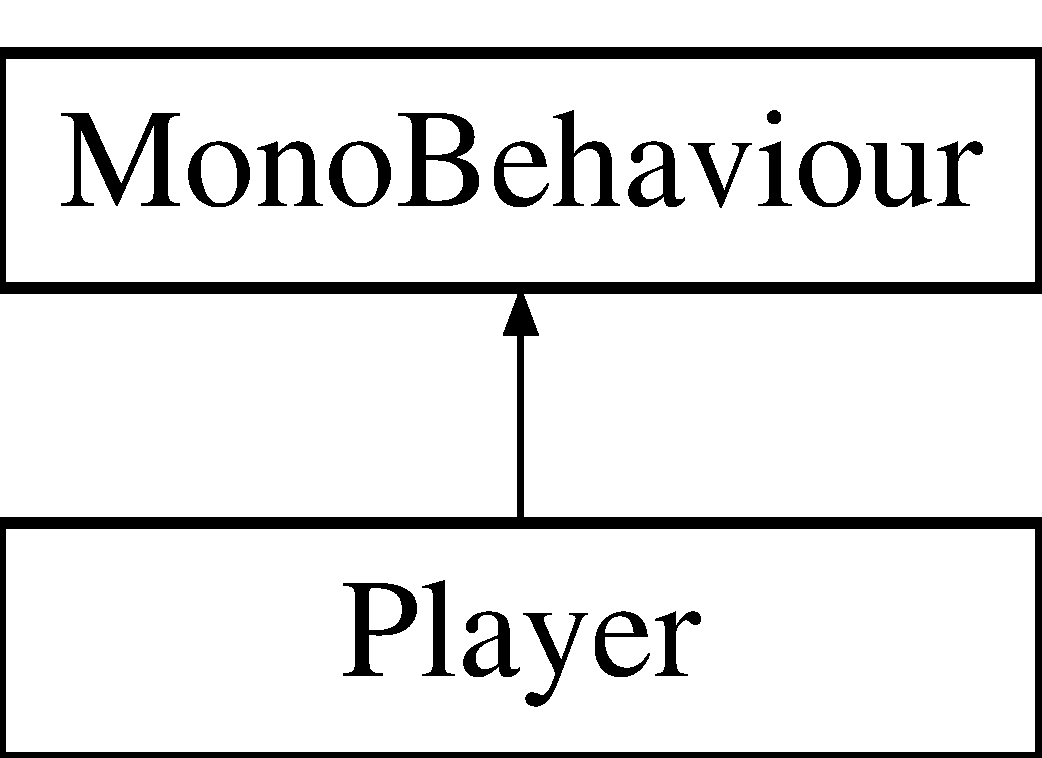
\includegraphics[height=2.000000cm]{class_player}
\end{center}
\end{figure}
\subsection*{Public Member Functions}
\begin{DoxyCompactItemize}
\item 
void \hyperlink{class_player_a1a09a3ded16ac1646f6bdd4f25fe0ddd}{Start} ()
\item 
void \hyperlink{class_player_aace80372e18e32fe177e295fe5d93ba8}{Update} ()
\begin{DoxyCompactList}\small\item\em Wywolywane dla kazdej klatki animacji gry. Wywolanie metody Handle\+Imput(), obslugujacej nacisniecie klawiszy przez gracza. Ustawiana jest predkosc w poziomie, zalezna od kierunku zwrotu gracza, oraz tego czy znajduje sie w powietrzu lub na ziemi. \end{DoxyCompactList}\item 
void \hyperlink{class_player_a6d893d1229110e7eb17eb7d895198717}{Handle\+Input} ()
\begin{DoxyCompactList}\small\item\em Obsluga interakcji gracza (nacisniecia klawisza A lub D), umozliwiajaca obrot. Nacisniecie spacji wykonuje skok. \end{DoxyCompactList}\end{DoxyCompactItemize}
\subsection*{Public Attributes}
\begin{DoxyCompactItemize}
\item 
float \hyperlink{class_player_a00cb3f26349dd5f58ad0a6135b763a07}{Max\+Speed} = 8
\begin{DoxyCompactList}\small\item\em Maksymalna liczba jednostek na sekunde, jakie gracz moze przejsc. \end{DoxyCompactList}\item 
float \hyperlink{class_player_ae1d47d3f4f67909f7498d900c1feedfa}{Speed\+Acceleration\+On\+Ground} = 10f
\begin{DoxyCompactList}\small\item\em Jak szybko moze zmienic sie predkosc gracza na ziemi. \end{DoxyCompactList}\item 
float \hyperlink{class_player_a6a71edc877a84d4f038fcc2b8e4f2843}{Speed\+Acceleration\+In\+Air} = 5f
\begin{DoxyCompactList}\small\item\em Jak szybko moze zmienic sie predkosc gracza w powietrzu \end{DoxyCompactList}\end{DoxyCompactItemize}


\subsection{Detailed Description}
klasa \hyperlink{class_player}{Player} 



\subsection{Member Function Documentation}
\hypertarget{class_player_a6d893d1229110e7eb17eb7d895198717}{}\index{Player@{Player}!Handle\+Input@{Handle\+Input}}
\index{Handle\+Input@{Handle\+Input}!Player@{Player}}
\subsubsection[{Handle\+Input()}]{\setlength{\rightskip}{0pt plus 5cm}void Player.\+Handle\+Input (
\begin{DoxyParamCaption}
{}
\end{DoxyParamCaption}
)}\label{class_player_a6d893d1229110e7eb17eb7d895198717}


Obsluga interakcji gracza (nacisniecia klawisza A lub D), umozliwiajaca obrot. Nacisniecie spacji wykonuje skok. 

\hypertarget{class_player_a1a09a3ded16ac1646f6bdd4f25fe0ddd}{}\index{Player@{Player}!Start@{Start}}
\index{Start@{Start}!Player@{Player}}
\subsubsection[{Start()}]{\setlength{\rightskip}{0pt plus 5cm}void Player.\+Start (
\begin{DoxyParamCaption}
{}
\end{DoxyParamCaption}
)}\label{class_player_a1a09a3ded16ac1646f6bdd4f25fe0ddd}
Jesli gracz jest obrocony, wartosc local\+Scale.\+x bedzie mniejsza od 0. \hypertarget{class_player_aace80372e18e32fe177e295fe5d93ba8}{}\index{Player@{Player}!Update@{Update}}
\index{Update@{Update}!Player@{Player}}
\subsubsection[{Update()}]{\setlength{\rightskip}{0pt plus 5cm}void Player.\+Update (
\begin{DoxyParamCaption}
{}
\end{DoxyParamCaption}
)}\label{class_player_aace80372e18e32fe177e295fe5d93ba8}


Wywolywane dla kazdej klatki animacji gry. Wywolanie metody Handle\+Imput(), obslugujacej nacisniecie klawiszy przez gracza. Ustawiana jest predkosc w poziomie, zalezna od kierunku zwrotu gracza, oraz tego czy znajduje sie w powietrzu lub na ziemi. 



\subsection{Member Data Documentation}
\hypertarget{class_player_a00cb3f26349dd5f58ad0a6135b763a07}{}\index{Player@{Player}!Max\+Speed@{Max\+Speed}}
\index{Max\+Speed@{Max\+Speed}!Player@{Player}}
\subsubsection[{Max\+Speed}]{\setlength{\rightskip}{0pt plus 5cm}float Player.\+Max\+Speed = 8}\label{class_player_a00cb3f26349dd5f58ad0a6135b763a07}


Maksymalna liczba jednostek na sekunde, jakie gracz moze przejsc. 

\hypertarget{class_player_a6a71edc877a84d4f038fcc2b8e4f2843}{}\index{Player@{Player}!Speed\+Acceleration\+In\+Air@{Speed\+Acceleration\+In\+Air}}
\index{Speed\+Acceleration\+In\+Air@{Speed\+Acceleration\+In\+Air}!Player@{Player}}
\subsubsection[{Speed\+Acceleration\+In\+Air}]{\setlength{\rightskip}{0pt plus 5cm}float Player.\+Speed\+Acceleration\+In\+Air = 5f}\label{class_player_a6a71edc877a84d4f038fcc2b8e4f2843}


Jak szybko moze zmienic sie predkosc gracza w powietrzu 

\hypertarget{class_player_ae1d47d3f4f67909f7498d900c1feedfa}{}\index{Player@{Player}!Speed\+Acceleration\+On\+Ground@{Speed\+Acceleration\+On\+Ground}}
\index{Speed\+Acceleration\+On\+Ground@{Speed\+Acceleration\+On\+Ground}!Player@{Player}}
\subsubsection[{Speed\+Acceleration\+On\+Ground}]{\setlength{\rightskip}{0pt plus 5cm}float Player.\+Speed\+Acceleration\+On\+Ground = 10f}\label{class_player_ae1d47d3f4f67909f7498d900c1feedfa}


Jak szybko moze zmienic sie predkosc gracza na ziemi. 



The documentation for this class was generated from the following file\+:\begin{DoxyCompactItemize}
\item 
C\+:/\+Users/\+Paul/\+Projects/\+Unity\+Game/\+Projekt/\+Assets/\+Code/Player.\+cs\end{DoxyCompactItemize}

\hypertarget{class_sort_particle_system}{}\section{Sort\+Particle\+System Class Reference}
\label{class_sort_particle_system}\index{Sort\+Particle\+System@{Sort\+Particle\+System}}


klasa \hyperlink{class_sort_particle_system}{Sort\+Particle\+System}  


Inheritance diagram for Sort\+Particle\+System\+:\begin{figure}[H]
\begin{center}
\leavevmode
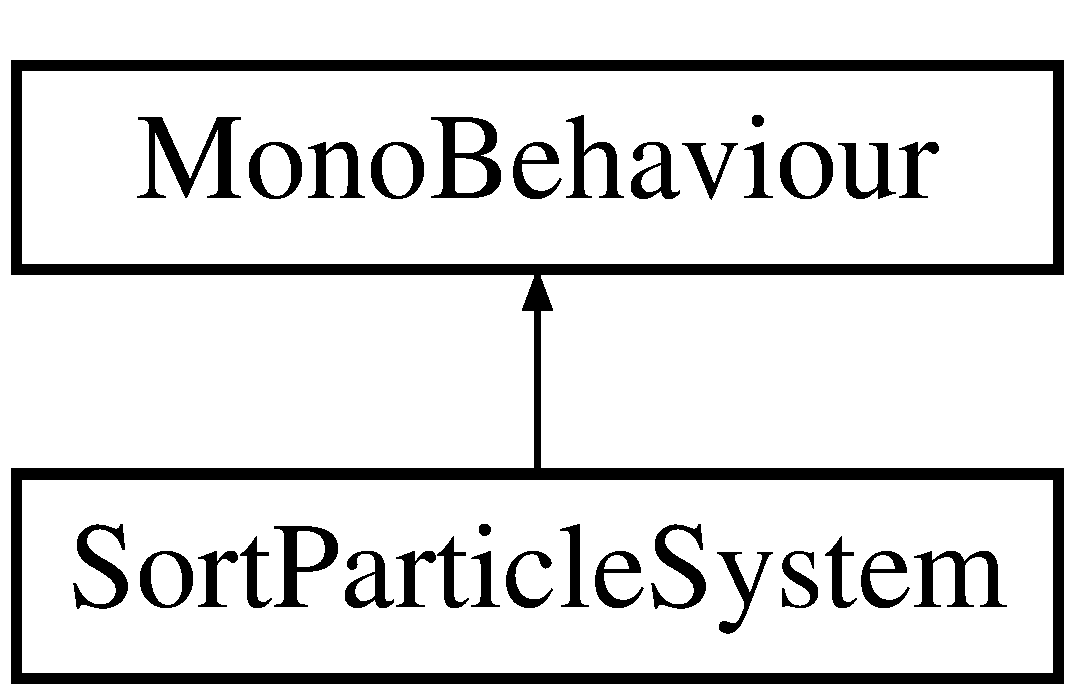
\includegraphics[height=2.000000cm]{class_sort_particle_system}
\end{center}
\end{figure}
\subsection*{Public Member Functions}
\begin{DoxyCompactItemize}
\item 
void \hyperlink{class_sort_particle_system_a671745a1f19ee8e655d8cd4ed2ccd06e}{Start} ()
\begin{DoxyCompactList}\small\item\em Domyślnie Particle\+System nie ma opcji ustawiania warstwy, na której ma być wyświetlany. \end{DoxyCompactList}\end{DoxyCompactItemize}
\subsection*{Public Attributes}
\begin{DoxyCompactItemize}
\item 
string \hyperlink{class_sort_particle_system_a9d51c7cdcf653de70767eef676bce85d}{Layer\+Name} = \char`\"{}Particles\char`\"{}
\begin{DoxyCompactList}\small\item\em Nazwa warstwy \end{DoxyCompactList}\end{DoxyCompactItemize}


\subsection{Detailed Description}
klasa \hyperlink{class_sort_particle_system}{Sort\+Particle\+System} 



\subsection{Member Function Documentation}
\hypertarget{class_sort_particle_system_a671745a1f19ee8e655d8cd4ed2ccd06e}{}\index{Sort\+Particle\+System@{Sort\+Particle\+System}!Start@{Start}}
\index{Start@{Start}!Sort\+Particle\+System@{Sort\+Particle\+System}}
\subsubsection[{Start()}]{\setlength{\rightskip}{0pt plus 5cm}void Sort\+Particle\+System.\+Start (
\begin{DoxyParamCaption}
{}
\end{DoxyParamCaption}
)}\label{class_sort_particle_system_a671745a1f19ee8e655d8cd4ed2ccd06e}


Domyślnie Particle\+System nie ma opcji ustawiania warstwy, na której ma być wyświetlany. 



\subsection{Member Data Documentation}
\hypertarget{class_sort_particle_system_a9d51c7cdcf653de70767eef676bce85d}{}\index{Sort\+Particle\+System@{Sort\+Particle\+System}!Layer\+Name@{Layer\+Name}}
\index{Layer\+Name@{Layer\+Name}!Sort\+Particle\+System@{Sort\+Particle\+System}}
\subsubsection[{Layer\+Name}]{\setlength{\rightskip}{0pt plus 5cm}string Sort\+Particle\+System.\+Layer\+Name = \char`\"{}Particles\char`\"{}}\label{class_sort_particle_system_a9d51c7cdcf653de70767eef676bce85d}


Nazwa warstwy 



The documentation for this class was generated from the following file\+:\begin{DoxyCompactItemize}
\item 
C\+:/\+Users/\+Paul/\+Projects/\+Unity\+Game/\+Projekt/\+Assets/\+Code/Sort\+Particle\+System.\+cs\end{DoxyCompactItemize}

%--- End generated contents ---

% Index
\backmatter
\newpage
\phantomsection
\clearemptydoublepage
\addcontentsline{toc}{chapter}{Index}
\printindex

\end{document}
